

\documentclass{article}

\usepackage{multirow}
\usepackage{geometry}
 \geometry{
 a4paper,
 total={170mm,257mm},
 left=20mm,
 top=20mm,
 }
\usepackage{cite}
\usepackage{amsmath,amssymb,amsfonts,bbm,amsthm}
\usepackage{algorithm}
\usepackage{MnSymbol}
\usepackage{graphicx,tikz}
\usepackage{enumitem}
\usepackage{flushend}
\usepackage{textcomp,multicol}
\usepackage{xcolor,url,comment}
\usepackage{stfloats,comment,lscape}
\usepackage{float,flushend}
\usepackage{graphics,subcaption,nameref,tikz}


\usepackage{algpseudocode}

%\makeatletter
%\def\BState{\State\hskip-\ALG@thistlm}
%\makeatother
\renewcommand{\algorithmicrequire}{\textbf{Input:}}
\renewcommand{\algorithmicensure}{\textbf{Output:}}
%\algrenewcommand\algorithmicindent{.12em}
\let\oldReturn\Return
\renewcommand{\Return}{\State\oldReturn}
%\biboptions{comma,round}

% \biboptions{}

% if you have landscape tables
\usepackage[figuresright]{rotating}

% put your own definitions here:
\newtheorem{theorem}{Theorem}[section]
\newtheorem{corollary}{Corollary}
\newtheorem{lemma}[theorem]{Lemma}
\newtheorem{proposition}{Proposition}
\newtheorem{example}[theorem]{Example}
\newtheorem{remark}{Remark}
\newtheorem{definition}{Definition}[section]
\newcommand\fig{\includegraphics}
\newcommand\btab{\begin{tabular}}
\newcommand\etab{\end{tabular}}
\newcommand\bfig{\begin{figure}\centering}
\newcommand\efig{\end{figure}}
\newcommand\bfigs{\begin{figure*}\centering}
\newcommand\efigs{\end{figure*}}
\newcommand\R{\mathrel{R}}
\newcommand\A{\mathrm{AlgorithmAllocation}}
\newcommand\SMU{\mathrm{SumMemoryUsage}}
\newcommand\MU{\mathrm{MemoryUsage}}
\newcommand\TO{\mathrm{TotalOutput}}
\newcommand\CT{\mathrm{CompletionTime}}
\newcommand\Idle{\mathrm{Idle}}
\newcommand\idle{\mathrm{idle}}
\newcommand\bT{\mathbf{T}}
\newcommand\GT{\mathbf{GT}}
\newcommand\ICT{\mathbf{InvCommTime}}
\newcommand\ComT{\mathbf{CommTime}}
\usepackage{authblk}

\title{A Survey on Task Allocation and Scheduling in Robotic Network Systems}
\author[1]{Saeid Alirezazadeh\thanks{The work was done when Saeid Alirezazadeh was with C4-Cloud Computing Competence Center, Universidade da Beira Interior, C4-Estrada Municipal, 506, 6200-284, Covilh\~{a}, Portugal. He is now with Physikalische und Theoretische Chemie, Universit\"{a}t Graz, Heinrichstra\ss{}e 28, Graz, 8010, Austria.}}
\author[2]{Lu\'{i}s A. Alexandre}
\affil[1]{C4 - Cloud Computing Competence Centre (C4-UBI), Universidade da Beira Interior, Rua Marqu\^{e}s d'\'{A}vila e Bolama, 6201-001, Covilh\~{a}, Portugal}
\affil[2]{NOVA LINCS, Universidade da Beira Interior, Covilh\~{a}, Portugal.}
\affil[1]{Email id: saeid.alirezazadeh@gmail.com}
\affil[2]{Email id: lfbaa@di.ubi.pt}
\date{}
\renewcommand\Affilfont{\itshape\small}


\providecommand{\keywords}[1]{\textbf{\textit{Keywords---}} #1}
\begin{document}

\maketitle

\begin{abstract}
Cloud Robotics is helping to create a new generation of robots that leverage the nearly unlimited resources of large data centers (i.e., the cloud), overcoming the limitations imposed by on-board resources. Different processing power, capabilities, resource sizes, energy consumption, and so forth, make scheduling and task allocation critical components. The basic idea of task allocation and scheduling is to optimize performance by minimizing completion time, energy consumption, delays between two consecutive tasks, along with others, and maximizing resource utilization, number of completed tasks in a given time interval, and suchlike. In the past, several works have addressed various aspects of task allocation and scheduling. In this paper, we provide a comprehensive overview of task allocation and scheduling strategies and related metrics suitable for robotic network cloud systems. We discuss the issues related to allocation and scheduling methods and the limitations that need to be overcome. The literature review is organized according to three different viewpoints: Architectures and Applications, Methods and Parameters. In addition, the limitations of each method are highlighted for future research.
\end{abstract}

\keywords{cloud, fog, edge, robotic network, task allocation, scheduling, load balancing}

% For peer review papers, you can put extra information on the cover
% page as needed:
% \ifCLASSOPTIONpeerreview
% \begin{center} \bfseries EDICS Category: 3-BBND \end{center}
% \fi
%
% For peerreview papers, this IEEEtran command inserts a page break and
% creates the second title. It will be ignored for other modes.

\section{Introduction}
Robots can take on dangerous tasks, and act as helpful companions, and their use is rapidly increasing in all aspects of human life \cite{Chatterjee:2021, Amritha:2022}. Some tasks like carrying a very heavy object, monitoring a wide area or dealing with a disaster cannot be performed by a single robot. To overcome this limitation, several studies, such as \cite{osumi:2014, michael:2012, Hu:2012, McKee:2008, Mckee:2000, Tenorth:2013, Kamei:2012}, propose that multiple robots can be used to perform tasks cooperatively, in a configuration called a robotic network. The capacity of a robotic network is limited by the collective capacity of all robots, \cite{Hu:2012}. Increasing the number of robots can increase the capacity, but it also increases the complexity of the model. Moreover, most tasks related to human-robot collaboration, such as speech, face, and object recognition, are very computationally intensive.

To overcome the computational limitations of a robotic network, we can leverage cloud robotics by using the Internet and cloud infrastructure to assign computations and share Big Data in real time \cite{kehoe:2015}. An important factor in determining the performance of cloud-based robotic systems is deciding whether to upload a newly arrived task to the cloud, process it on a server (fog computing \cite{bonomi:2012}), or execute it on one of the robots (edge computing \cite{shi:2016}), which is called the allocation problem. When the allocation problem is solved, the result is a set of tasks assigned to each processing unit. The scheduling problem deals with the problem of arranging (scheduling) this set of tasks, given the priority of the tasks, their time constraints, and the precedence order among the tasks, to answer the question of which task, from the set of tasks assigned to each processing unit, should be executed first.

We assume that the system can only perform a finite set of tasks $T$ and that over time a set of tasks $T_i$, a subset of $T$, arrives that must be performed by the system. Figure \ref{fig0} shows an overview of the approaches to task allocation.

\begin{figure*}[tb]\centering
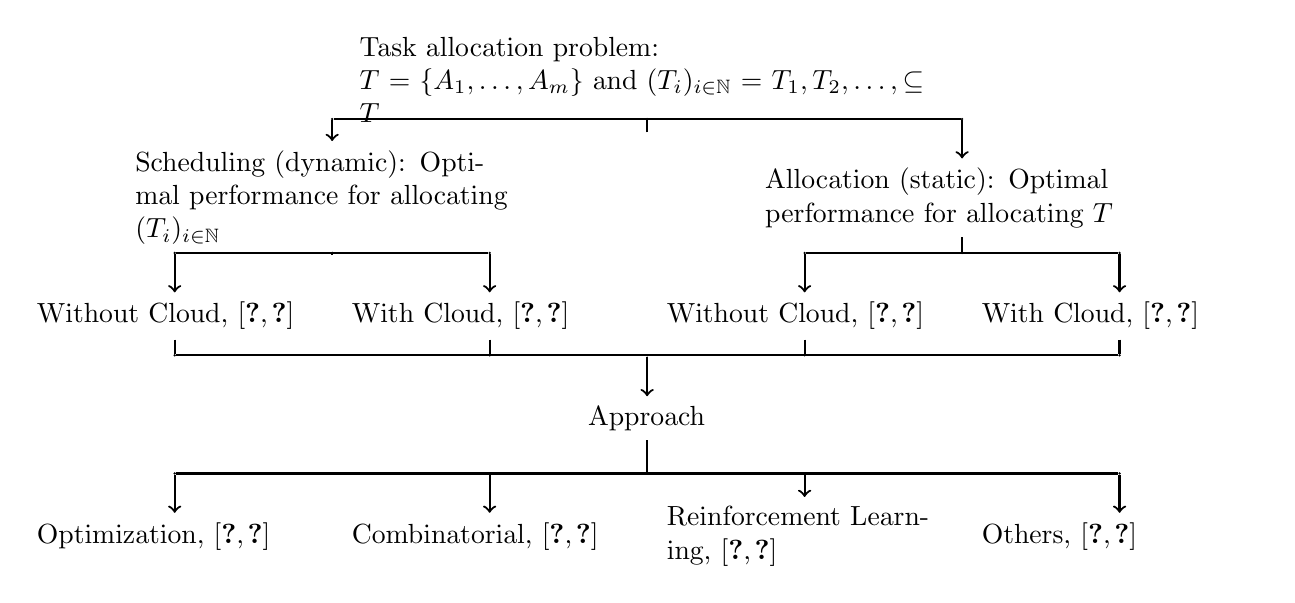
\begin{tikzpicture}
\begin{scope}%[every node/.style={rectangle,thick,draw,rounded corners=.8ex}]
    \node (A) at (0,0) [text width=7.3cm] {Task allocation problem: \\$T=\{A_1,\ldots,A_m\}$ and  $(T_i)_{i\in\mathbb{N}}=T_1,T_2,\ldots, \subseteq T$};
    \node[fill,circle,scale=0.1]  (B) at (0,-0.5) {};
    \node[fill,circle,scale=0.1]  (C) at (-4,-0.5) {};
    \node[fill,circle,scale=0.1]  (D) at (4,-0.5) {};
    \node (E) at (-4,-1.5)  [text width=5cm] {Scheduling (dynamic): Optimal performance for allocating $(T_i)_{i\in\mathbb{N}}$};
    \node (F) at (4,-1.5)  [text width=5cm] {Allocation (static): Optimal performance for allocating $T$};
    \node[fill,circle,scale=0.1]  (G) at (-4,-2.2) {};
    \node[fill,circle,scale=0.1]  (H) at (-6,-2.2) {};
    \node[fill,circle,scale=0.1]  (I) at (-2,-2.2) {};
    \node[fill,circle,scale=0.1]  (J) at (4,-2.2) {};
    \node[fill,circle,scale=0.1]  (K) at (2,-2.2) {};
    \node[fill,circle,scale=0.1]  (L) at (6,-2.2) {};
    \node (M) at (-6,-3) [text width=3.5cm] {Without Cloud, \cite{Ours:2022ral, Sa:2021}};
    \node (N) at (-2,-3) [text width=3.5cm] {With Cloud, \cite{Shafiq:2021, Bharti:2022}};
    \node (O) at (2,-3) [text width=3.5cm] {Without Cloud, \cite{Fu:2021,Orr:2020}};
    \node (P) at (6,-3) [text width=3.5cm] {With Cloud, \cite{Minjia:2021,Pu:2021}};
    \node[fill,circle,scale=0.1]  (Q) at (-6,-3.5) {};
    \node[fill,circle,scale=0.1]  (R) at (-2,-3.5) {};
    \node[fill,circle,scale=0.1]  (S) at (2,-3.5) {};
    \node[fill,circle,scale=0.1]  (T) at (6,-3.5) {};
    \node[fill,circle,scale=0.1]  (U) at (0,-3.5) {};
    \node (V) at (0,-4.3) [text width=1.5cm] {Approach};
    \node[fill,circle,scale=0.1]  (W) at (0,-5) {};
    \node[fill,circle,scale=0.1]  (X) at (-6,-5) {};
    \node[fill,circle,scale=0.1]  (Y) at (-2,-5) {};
    \node[fill,circle,scale=0.1]  (Z) at (2,-5) {};
    \node[fill,circle,scale=0.1]  (a) at (6,-5) {};

    \node (b) at (-6,-5.8) [text width=3.5cm] {Optimization, \cite{Bai:2022,Ours:2022net}};
    \node (c) at (-2,-5.8) [text width=3.5cm] {Combinatorial, \cite{Jin:2022,Bharti:2022}};
    \node (d) at (2,-5.8) [text width=3.5cm] {Reinforcement Learning, \cite{Bian:2019,Ding:2020}};
    \node (e) at (6,-5.8) [text width=3.5cm] {Others, \cite{Ours:2022ral,Ours:2020h}};


\end{scope}

    \path [->] (A) edge[thick,-] (B);
    \path [->] (C) edge[thick,-] (D);
    \path [->] (E) edge[thick,-] (G);
    \path [->] (F) edge[thick,-] (J);
    \path [->] (H) edge[thick,-] (I);
    \path [->] (K) edge[thick,-] (L);
    \path [->] (M) edge[thick,-] (Q);
    \path [->] (N) edge[thick,-] (R);
    \path [->] (O) edge[thick,-] (S);
    \path [->] (P) edge[thick,-] (T);
    \path [->] (Q) edge[thick,-] (T);
    \path [->] (V) edge[thick,-] (W);
    \path [->] (X) edge[thick,-] (a);


    \path [->](C) edge [thick,->] (E);
    \path [->](D) edge [thick,->] (F);
    \path [->](H) edge [thick,->] (M);
    \path [->](I) edge [thick,->] (N);
    \path [->](K) edge [thick,->] (O);
    \path [->](L) edge [thick,->] (P);
    \path [->](U) edge [thick,->] (V);
    \path [->](X) edge [thick,->] (b);
    \path [->](Y) edge [thick,->] (c);
    \path [->](Z) edge [thick,->] (d);
    \path [->](a) edge [thick,->] (e);

\end{tikzpicture}
\caption{Overview of the task allocation approaches.}
\label{fig0}
\end{figure*}

Allocation and scheduling problems usually involve optimizing one or more parameters such as time, total energy consumption, total resource consumption, average memory usage, etc., for completing all tasks. If the problem is limited only to the use of a cloud server, parameters such as load balancing and minimizing the makespan should be considered.

All articles that contained the word "scheduling" and/or "allocation" in the title or keyword and were published between 2017 and 2022 were first selected from high-ranking scientific journals and conferences. Studies were selected that addressed the problem in robotic networks or in the cloud. We tried to cover most of the methods used in recent studies.

In the article \cite{Arunarani:2019}, articles related to scheduling in cloud computing were examined. The authors examined all articles with the word ''scheduling'' in the title or keyword published from January 2005 to March 2018. The article explains the importance of task scheduling, and that it cannot be done manually. The main benefits of proper task scheduling are: (for the user) spending less money on using virtual machines, getting the result of task execution faster, among others, and (for the cloud provider) processing a large number of incoming requests, spending less on service maintenance, providing the best quality of service, and so forth. Existing task scheduling techniques have been classified into ten categories: QoS-based task scheduling, Ant Colony Optimization Algorithm-based task scheduling, PSO-based task scheduling, Genetic Algorithm-based task scheduling, Multiprocessor-based task scheduling, Fuzzy-based task scheduling, Clustering-based task scheduling, Deadline-constrained scheduling, Cost-based task scheduling, and other scheduling-based approaches. They briefly explain each category with its advantages and limitations. They categorize the papers according to the year of publication, the techniques and parameters they measure, and state their limitations and highlighted time complexity. Several studies mainly focus on scheduling and task allocation without considering the cloud infrastructure. These methods can be combined with studies on scheduling in cloud computing so that the result is useful for a wider range of audiences. The paper \cite{Arunarani:2019} focuses mainly on works on cloud computing and works that apply scheduling methods to robotic networks are not included. Scheduling methods are also evolving rapidly, and several new methods have been developed in the last four years.

The authors of the article \cite{Rizk:2019} examined studies on heterogeneous multiagent systems and focused mainly on robot agents. They considered studies on task decomposition, coalition formation, task allocation, and multiagent scheduling. Most studies dealing with cloud infrastructures have not considered optimal task allocation in the cloud. The automation of the task allocation problem is divided into three stages depending on the amount of usages of human agents to find an optimal task allocation. Finally, task decomposition, coalition formation, and task allocation are considered separately. Several challenges such as using Big Data, considering task complexity, applying machine learning, human-robot collaboration, and communication instability are identified for further exploration. Most of these challenges have been explored in recent years and several results have been proposed.

The review article \cite{Dawarka:2022} examined the studies on the cloud robotic architecture developments without considering task allocation and scheduling, which is beneficial for further optimizing the performance of a cloud robotic system.

\section{Categorization}

We present high level view of the works as charts according several distinguishing figures in Figure \ref{fig1}. %to the year of publication (Figure \ref{fig1}), according to their content: static or dynamic (Figure \ref{fig2}), considering the cloud (Figure \ref{fig3}), the number of robots (Figure \ref{fig4}), load balancing (Figure \ref{fig5}), human-robot collaboration (Figure \ref{fig6}), and according to the approach used to find the solution (Figure \ref{fig7}).
\begin{figure}
     \centering
     \begin{subfigure}[b]{0.3\linewidth}
         \centering
         \includegraphics[width=1\linewidth]{p1.pdf}
         \caption{Categorizing by year.}
     \end{subfigure}
     \hfill
     \begin{subfigure}[b]{0.3\linewidth}
         \centering
         \includegraphics[width=1\linewidth]{p2.pdf}
         \caption{Categorizing by being static or dynamic task assignment.}
     \end{subfigure}
     \hfill
     \begin{subfigure}[b]{0.3\linewidth}
         \centering
         \includegraphics[width=1\linewidth]{p3.pdf}
         \caption{Categorizing by considering cloud or not.}
     \end{subfigure}
     \hfill
     \begin{subfigure}[b]{0.3\linewidth}
         \centering
         \includegraphics[width=1\linewidth]{p4.pdf}
         \caption{Categorizing by number of robots.}
     \end{subfigure}
     \hfill
     \begin{subfigure}[b]{0.3\linewidth}
         \centering
         \includegraphics[width=1\linewidth]{p5.pdf}
         \caption{Categorizing by aiming to balance the loads.}
     \end{subfigure}
     \hfill
     \begin{subfigure}[b]{0.3\linewidth}
         \centering
         \includegraphics[width=1\linewidth]{p6.pdf}
         \caption{Categorizing by considering human-robot collaboration.}
     \end{subfigure}
     \hfill
     \begin{subfigure}[b]{0.3\linewidth}
         \centering
         \includegraphics[width=1\linewidth]{p7.pdf}
         \caption{Categorizing by the approach used to solve the problem.}
     \end{subfigure}\hfill
        \caption{Different categorization of all contributions.}
        \label{fig1}
\end{figure}

All contributions have been considered by:
\begin{itemize} 
\item Year: publication year of a developed model.
\item Static/Dynamic: there are two ways to assign tasks to processing units: static, which answers the question of how to achieve optimal system performance by assigning tasks in the set of all tasks that can be executed by the processing units of a given system architecture, and dynamic, which answers the question of how to achieve optimal system performance by assigning tasks dynamically in the order of the sets of arrived tasks by time. 
\item Load balancing: the scheduling model that describes a method in which all processing units complete their tasks at nearly the same time.
\item Cloud infrastructure: whether or not a scheduling model is described for a system architecture with cloud infrastructure.
\item Number of robots: number of robots used in the system architecture.
\item Parameters: The list of all parameters used to develop a model for the sceduling and task allocation problem.
\item Main objectives: The main objective of the developed model.
\item Approach Used: The approach used to describe the model and the method used to solve the problem.
\item Restrictions: The list of constraints on a developed model that should be considered before using or adapting it to other extended problems.
\item Problems: The list of problems that need to be further investigated in a developed model that could not be answered by the current model.
\item Type of Experiments: The type of experiments used to test and validate the developed model: simulation or real-world test.
\end{itemize}

We classify the papers by their solution approach to scheduling and task allocation, and then sort them by the year they were published. The list of solution approaches are: 
\begin{itemize}
\item Optimization: the scheduling and allocation problem is translated into an optimization model and a solution to it is described.
\item Combinatorial: the scheduling and allocation problem is translated into a graph-theoretic or set-theoretic model and a solution for it is described.
\item Reinforcement Learning: the scheduling and allocation problem is translated into a model that is solved by a reinforcement learning approach.
\item Others: the scheduling and allocation problem is translated into another model and a solution for it is described, such as a language and automata model, a geometric model, or the development of a new architecture.
\end{itemize}
All contributions are summarized in Appendix \nameref{summary} based on their solution approachs.

\section{Optimization}
In this section we discuss contributions that solve the problem using an optimization problem and apply a standard solver to obtain the result. The works are separately analyzed based on whether the cloud infrastructure is considered or not.
\subsection{Without Cloud}
\cite{Gini:2017} proposed an optimization approach that can be solved by several possible methods, such as market-based, swarm-based, distributed constraint optimization methods as a decentralized approach or branch-and-bound method as a centralized approach to minimize a cost function or maximize a reward function for all robots for completing their tasks. The temporal model is translated into logical expressions, \cite{Allen:1983}, and then the logical expression is translated into a graph that facilitates its use, \cite{DECHTER:1991}. Dynamic task allocation is used in modeling systems with environmental changes. Depending on which model (centralized or decentralized) is chosen, different solutions are proposed: branch-and-bounds or metaheuristics for the centralized model and distributed constraint (DCOP)-based methods or market-based methods for the decentralized model. 

%\textbf{Taxonomy:} Dynamic task allocation of a robotic network minimizing the task completion time by robots.

%\textbf{Limitations and Future work:} 
In this approach, all robots in the decentralized model should be able to communicate with each other and in the centralized model, the central unit should be able to communicate with all robots. Moreover, communication failures have not been considered, which means that in the centralized model, the central unit has to reschedule all tasks and generate new solutions when new tasks arrive, while in the decentralized model, approximation methods should be used to reduce the computation time. Moreover, robots that can perform multiple tasks simultaneously and multi-robot tasks are not considered, and disjoint temporal models are not considered.

\cite{NUNES:2017} studied the ordering of tasks with time window constraints. They described a general optimization model for the task allocation problem from which all existing methods can be derived by considering a general optimization of a generic function, which can be a cost function, a reward, a distance to the task, etc., and then, depending on the problem, maximize the number of tasks completed, minimize the sum of the total path cost of all robots, minimize the latency, maximize the reward, and minimize the number of robots deployed. 

%\textbf{Taxonomy:} General optimization problem of dynamic task allocation of a robotic network.

%\textbf{Limitations and Future work:} 
The time constraints are simple and time-critical tasks cannot be correctly assigned to robots. To find a solution, they investigated various existing solutions according to the main problem by considering the centralized and the distributed solution methods, but there is no clear way to solve problems with multiple objectives.

\cite{LEE:2018} investigated the optimization of task completion time, resource consumption, and communication time. The author proposed a resource-based task allocation method to ensure the efficiency of task allocation over a long period of time. The proposed task allocation method is a market-based approach. And it assumes that occasional recharge and resources are consumable resources available to robots in task allocation, which includes rescheduling of tasks. 

%\textbf{Taxonomy:} Dynamic task allocation of robotic network minimizing the task completion time, resource consumption and communication time by robots.

%\textbf{Limitations and Future work:} 
The method does not consider the two parameters recharge time and transfer time to recharge stations, which may change the solution. Moreover, their method is compared with the cases without task rescheduling and without considering resources. To improve performance, additional constraints are introduced into the optimization problem and performance is experimentally compared to methods without considering the additional constraints. However, the improved performance is apparent even without testing.

\cite{Zhou:2018} developed a method that finds the smallest number of robots in a given time limit and assigns tasks to them so that the robots can complete their tasks within the time-limit. The authors proposed a multi-objective approach called Mofint (multi-objective GA with forest individual containing non-intersecting trees), which first finds upper and lower bounds on the number of robots and then determines the optimal completion time by finding an optimal spanning forest. The main problem they addressed is the complete coverage problem (CCP), which is equivalent to finding an optimal spanning forest in graph theory \cite{Pettie:2008, Hell:1985}. The problem is to find the smallest path that avoids obstacles between all points in a given area. First, an area is divided into several regions with respect to obstacles. Each region is considered as a task, and each task is assigned to a robot. Considering the regions as vertices and adjacent regions as edges, a graph is obtained. Given a number of robots, the solution to the coverage problem (minimum completion time) with a given number of robots is to find the optimal spanning forest where the number of tree components equals the number of robots. Since the regions of the area are a partition of the area and each region is assigned to a robot, there is no overlap between the robots. The method for finding the regions is partitioning and homomorphic projection using Morse theory \cite{Milnor:1963}, where the area becomes a union of different bands. Next, they find the upper and lower bounds on the number of robots. Then, from the lower bound (LB) to the upper bound (UB), they test whether the completion time is shorter than the time limit. For the bounds, the LB for a fixed number of regions is equal to the smallest integer greater than or equal to the value of the sum of all weights divided by the time limit. For the UB, generate a random spanning tree and then use the linear tree partitioning algorithm to determine the number of partitions. In this algorithm, the random spanning tree is partitioned into multiple parts such that the sum of the weights of all parts is less than or equal to the time limit. The objective is then to minimize the weight of the heaviest tree in the spanning forest. To solve the optimization problem, randomly create a forest with a fixed number of trees between the LB and the UB. And then add random edges to create a LB-tree forest. 

%\textbf{Taxonomy:} Dynamic task allocation for finding minimum number of robots to be able to complete a task within a time limit.

%\textbf{Limitations and Future work:} 
The weights of the vertices of the graph of regions are considered as non-negative integers. Since we are looking for the minimum number of robots, we should look for an appropriate partition for this number of robots. Such a partition should be defined in such a way that it does not exceed the time limit. Moreover, the definition of the band size depends on the metric, which is not defined. Next, the UB can be defined simply as the number of vertices determined by the partitioning of the region. Moreover, the partitioning of vertices into a fixed number of parts is not unique. Examples can be found where the region is partitioned into a fixed number of parts such that one part meets the time limit but another part does not, see Figures \ref{figu12} and \ref{figu13}. Therefore, the assignment of each partition of nodes to robots does not necessarily mean that it does or does not respect the time limit. To solve the optimization problem by adding random edges that either create a cycle or reduce the number of trees by one, we need to check for possible cycles in the graph after adding each random edge.

\begin{figure}[th!]
\begin{minipage}{.48\textwidth}
\centering
\includegraphics[width=0.42\linewidth]{P11.png}
\caption{Environment abstraction. The imaginary vertical dashed lines are some borders of regions, $v_1$ to $v_5$. The filled object in the middle of the environment is the obstacle.} 
\label{figu12}
\end{minipage}\hfill
\begin{minipage}{.48\textwidth}
\centering
\includegraphics[width=.9\linewidth]{P12.png}
\caption{Task allocation. Two possible allocation to three robots. Tasks for each robot can form a spanning tree. The partitioning vertices in the left will pass the time limit, $T=2$, but the right one does not pass the time limit.} 
\label{figu13}
\end{minipage}
\end{figure}

\cite{Dantu:2019} studied distributed dynamic task assignment algorithm for swarms of robots under the assumption of communication instability. The problem is translated into an optimization problem for maximizing the utility of all agents. In order to solve the optimization problem, it is necessary to maintain the bundle vector (the list of tasks assigned to the agents, where the tasks are ordered by when they were won), the path vector (the same as the bundle vector, but the order of tasks is the order in which the tasks are completed by the respective agents), the winning agent vector (the vector of values corresponding to the agents and tasks to determine an agent's expectation of which agent placed the highest bid on the task), the winning bid vector (the vector of values corresponding to the agents and tasks to determine an agent's expectation of placing the highest bid among all agents on the task), and the timestamp vector (the vector of values corresponding to the agents and tasks to determine when an agent placed the bid on the task). 

%\textbf{Taxonomy:} Dynamic task allocation of a robotic network minimizing the task completion time by robots.

%\textbf{Limitations and Future work:} 
In the case where all tasks have relatively long execution times with respect to the average communication time, communication delays do not lead to significant changes in the allocation. Moreover, the optimization problem can be simplified and transformed into linear programming by transforming the main objective logarithmically. And then the main objective is to minimize the completion time of all tasks instead of solving a more complex objective function.

\cite{Notomista:2019} examined capabilities and energy consumption by minimizing the cost function. In this study, the tasks are prioritized based on the time constraints and capabilities of the robots and the optimization problem (Mixed Integer Quadratic Problem) is solved to find the optimal task allocation. The optimal task allocation is achieved by updating the priorities of the tasks according to time. 

%\textbf{Taxonomy:} Dynamic task allocation of a robotic network minimizing the energy consumption by robots.

%\textbf{Limitations and Future work:} 
The cost function must belong to class $C^1$ (functions that are continuously differentiable), which is not specified in the paper, otherwise the arguments are not valid. Moreover, for each robot, the task with the highest priority is considered unique. Moreover, all the cost functions in the experimental results and examples are the distance to a certain point in a compact Euclidean subspace is a very simple function, but other cost functions such as a combination of energy consumption, time to complete tasks and some others can be considered which increase the complexity of the optimization problem. In some scenarios, where the cost functions are not of class $C^1$, the method cannot be applied. This means that their proposed method works only for special cost functions. For example, functions such as $|2x^2-1|$ or $|\frac{2}{\pi}\arctan(\frac{\pi}{2}x)|$ are not compatible with the application of their method. Moreover, their method does not take into account environmental changes.

\cite{emam:2020} studied the minimization of the cost function in a dynamic environment where task priorities may change due to environmental changes. The proposed method is similar to that of \cite{Notomista:2019}. The optimal allocation is achieved by updating the states of the robots over time and the priorities are updated with the changes in the environment. 

%\textbf{Taxonomy:} Dynamic task allocation of a robotic network in a dynamic environment minimizing the energy consumption by robots.

%\textbf{Limitations and Future work:} 
The cost function is considered to be continuously differentiable and for each robot, the task with the highest priority should be unique, which cannot cover more general scenarios. Moreover, it does not consider the scenario that an environmental disturbance can reduce the cost, e.g., removing an obstacle. Also, the frequency of environment changes must be considered, e.g., repeated placement and removal of obstacles in the same location.

\cite{Rahmanpour:2020} proposed a method for planning the motion and communication strategies for a robotic network to perform all tasks with the goal of minimizing energy consumption and avoiding collisions. For each task, a robot is selected, which is called the leader. The leader plans the movements to a particular location and when the task is completed for the newly arrived task based on the current formation, a new leader is selected. Each robot solves a convex optimization problem to plan a collision-avoiding optimal trajectory and an optimal communication strategy that guarantees network connectivity in the presence of uncertain communication. If we consider an agent (node) called an operations center (OC), it is an interconnected node that enables communication among all nodes. When a task is assigned to the team, a particular robot is selected as the leader. The leader will visit the task location within a certain time, and the other robots will support the leader by passing their information to the OC. To select the leader and configure the other robots, the robots search for the shortest obstacle-free path between OC and the task location after a task at that location is announced by OC. The shortest path is defined by a sequence of straight lines between the two positions in the flat surface of the area, where the line has no intersection with obstacles. This path is divided into several (number of robots) segments of equal length. Now the shortest (obstacle-free) path from the current position of each robot to each spot of the segments is found. This information is transmitted to all the robots, and then the robot is assigned to each spot in such a way that the total length of the path that the robots have to travel to reach that spot is minimal. In this way, we can minimize the movements of the robots to design the path from OC to the position of the task. 

%\textbf{Taxonomy:} Dynamic task allocation of a moving robotic network minimizing the energy consumption by robots, motion planning and collision avoidance.

%\textbf{Limitations and Future work:} 
Dynamic obstacles were not considered. In addition, the method for finding the shortest path should consider the case where there are two robots, both of which have identical minimum distances to the spots, and one is randomly selected. Moreover, the optimal assignment of robots to each segment cannot be found simply by finding the shortest path to each segment, see Figure \ref{figu8}. There are several examples where a robot should be assigned to a spot even though other robots are closer to that spot, see Figure \ref{figu9}. In addition, to find the optimal assignment of robots to spots, we need to solve the problem of minimizing the total paths traveled by all robots to each segment spot. The constraint on the threshold radius around the robots is not considered, which means that the size of the shortest distance between OC and the task for a given number of robots cannot be smaller than twice the sum of the radii around all robots; otherwise, we should use a smaller number of robots.

\begin{figure}[tbp]
\begin{minipage}{.48\textwidth}
\centering
\includegraphics[width=0.6\linewidth]{P1.png}
\caption{Three robots, where two of them (red and blue dots) have identical distance to all the spots $z_{h,v}$.}
\label{figu8}
\end{minipage}\hfill
\begin{minipage}{.48\textwidth}
\centering
\includegraphics[width=0.76\linewidth]{PP2.png}
\caption{An example of the obstacle-free path from the OC to the task, with 4 robots shown in color circles.}
\label{figu9}
\end{minipage}
\end{figure}

\cite{Brown:2020} studied the allocation and routing of robots to move objects between stations in such a way that the makespan (the time from start to finish) is minimal. The problem is translated into a problem called precedence constrained multi-agent task assignment and path-finding (PC-TAPF), which is an optimization problem to minimize the makespan. A hierarchical algorithm is proposed to find the optimal makespan. The proposed method jointly considers task dependencies, performs task scheduling, and provides routing that avoids collisions. The main idea is to solve the problem first without considering collisions. Then, the task assignment is passed to the so-called conflict-based search (CBS), which searches for the collision-free set of paths. Traveling Salesman method is used for the first part, and tree search is used for the second part. A 2D environment with multiple stations is considered, i.e., places where operations are performed on objects that are regularly placed at fixed positions. The stations contain pick-up and drop-off areas, i.e., places where objects are collected or dropped off before and after performing operations. There are also several robots that move objects from one station to another, where the position of each robot is known at a given time. The stations are the area where the robots cannot move. The position of each object at each point in time is known. It is assumed that a robot can pick up an object if the object and the robot have the same position at the same time. To avoid conflicts, the method looks for possible conflicts in the solution. If there is a conflict, the same is applied for the second time, but in this case, since the number of conflicts is already known, the nodes where there is a conflict are searched and their route is replaced by a conflict-free route. The proposed method consists of a four level algorithm. The sequential next-best assignment search (NBS) tries to find a valid operating schedule for a sequential assignment problem, the conflict-based search (CBS) uses a binary tree search to find an optimal path, incremental slackprioritized search (ISPS) obtains the operating schedule and set of constraints from CBS, slack and collisionaware tie-breaking $A^*$ ($A^*_{ SC }$) searches the graph to find the states corresponding to the critical path with the lowest cost. 

%\textbf{Taxonomy:} Dynamic task allocation of a moving robotic network minimizing the completion time by robots, motion planning and collision avoidance.

%\textbf{Limitations and Future work:} 
Saying that the object and the robot have the same position at the same time is not enough as a condition for an object to move. There should be a condition that specifies which of the robots that do not carry objects should move towards an object to carry it. For example, the concept of total distance between robots and objects can be introduced, which should be minimized for optimal scheduling of objects for the robots. Analogous to the existence of the final station (terminal), there should also be an initial station that has no inputs but produces several outputs (raw materials) that are used as inputs by other stations. Otherwise, these raw materials would have to be placed randomly in space. Moreover, since the proposed method does not impose any constraints on conflict avoidance, we cannot ensure that we will find a conflict-free route the second time. For example, there could be a node whose state in the route is conflict-free, but its state causes conflicts at other nodes, see Figure \ref{figu2}. This means that conflict avoidance should be added to the proposed algorithm in the first place. From the experimental results, we can conclude that ISPS is very fast. But as explained in , ISPS gets the set of constraints from CBS, and CBS gets the operating schedule from NBS. This means that the runtime of ISPS must always be higher than that of NBS. However, in the results, it is smaller than the runtime of NBS most of the time. The obtained runtime measurement is valid only if the algorithms are computed independently. However, this contradicts the proposed method which states that the algorithms must be executed with respect to each other. Since the goal is to minimize the makespan, there should be a result that gives the average makespan of each experiment.

\begin{figure}[h]\centering
\includegraphics[width=0.3\linewidth]{P4.png}
\caption{Nine robots are planned to move. Eight planned initially with the movement without conflict, but for the middle robot there is always conflict with other robots.}
\label{figu2}
\end{figure}

\cite{Behrens:2020} described an optimization problem for assigning tasks to robots in a sequence of tasks and motions of robots such that there are no collisions between robots, the predefined set of constraints is satisfied, and overall makespan is minimized. In their method, tasks are divided into confined tasks (a task where a robot's action is limited to a small part of the workspace, e.g., grasping and placing) and extended tasks (a task where a robot's action is limited to a large part of the workspace, e.g., welding along a line). The main focus is on the optimization of the extended tasks. For a given set of tasks that satisfy the set of constraints during execution, each task has multiple starting positions (called degrees of freedom), and the time interval in which a robot can perform each task is measured. The workspace is partitioned to identify regions that a robot occupies during the execution of a task in a sequence of time frames by discretizing the time interval of the task into smaller successive intervals. For solving tasks and motion planning for extended tasks, the problem is translated into a constraint satisfaction problem, which is a type of optimization problem modeled with triples $(X,D,C)$, where $X$ is a set of variables, $D$ is a set of domains where parameters take values, and $C$ is a set of constraints. The solution is to assign values from $D$ to the variables $X$ such that the set of all constraints $C$ is satisfied. To solve the problem, the gradient method and steepest descent by Cauchy \cite{Goldstein:1962} is used (backtracking search method), that is, start with an upper bound on the minimum makespan and add the constraint that the minimum makespan is less than the upper bound. Then, remove the values from the domains that do not satisfy the new constraint, and then decrease the value of the upper bound until the optimal solution is reached for the values of the variables. The optimization model is viewed from three perspectives: task layer, robot layer, and collision-free plan. 

%\textbf{Taxonomy:} Dynamic task allocation of a moving robotic network with two robots minimizing the completion time by robots, motion planning and collision avoidance.

%\textbf{Limitations and Future work:} 
The time intervals considered in the paper depend only on the task and the dependence on the robots is not considered, i.e., the robots should be identical. Moreover, the size of the region and the discretization of the time interval are not fixed and can be either a short or a long interval. Depending on the choice of the interval size and the size of the domain, different solutions can be obtained. Moreover, in the backtracking search method, in order to obtain a solution for the first upper bound, a random selection seems to be made in the solution space, so that the values in the domains that satisfy the constraints are selected. But the steps to reduce the upper bounds are not described. And the solution completely depends on the selection and reduction of the upper bounds. Moreover, different upper bounds may lead to different solutions. Also, the robot dependency is skipped but should be considered since the navigation codes, time intervals, constraints, and active components are robot-dependent, and their values may change when switching from one robot to another. In \cite{Behrens:2020}, tasks are translated into ordered visit constraints originally defined in \cite{Behrens:2019}. Here, the tasks are considered confined, so the start and end locations are considered identical, and the robot configuration is the same at the start and end. However, the new modified version includes different locations and different configurations to include extended tasks. Moreover, collisions may occur between components of a single robot, which is not considered. In addition, collision avoidance depends on the size of the regions (voxelization sizes). When the region size is large, the robots can have intersections in the configuration spaces, but when the region size is smaller, they have empty intersections, see Figure \ref{figu1} for a 2D example. This is consistent with the well-known result that there are always infinitely many other real numbers between two distinct real numbers, see \cite{Gaughan:1993}. This means that if the two robots are not connected at any point, there will always be a voxel size where the intersection of their voxalizations is empty.

\begin{figure}[th!]\centering
\includegraphics[width=0.8\linewidth]{P2.png}
\caption{Two robots space occupancy. With larger pixel size they have collision but with smaller pixels they do not have collision. The workspace is the large square. Pixel sizes are chosen as proportion of the total size with the factors $2^{-n}$ for $n=0,1,3,4$. The grey rectangles are pixels with robot collisions.} 
\label{figu1}
\end{figure}

\cite{Fu:2021} proposed a method to decide whether to assign subtasks to edge devices or offload them to fog nodes, such that the total execution time of all subtasks and the total energy consumption of all edge devices are minimal. In this method, the tasks that need to be executed by edge devices are translated into a DAG generated by the dependencies of the subtasks. Considering the average execution time and energy consumption of all subtasks on each core of the system architecture, the problem is then transformed into an optimization problem whose solution allows optimal scheduling of the subtasks. 

%\textbf{Taxonomy:} Dynamic task allocation of a robotic network minimizing the completion time and energy consumption by robots.

%\textbf{Limitations and Future work:} 
In this model, all edge devices must have a direct communication link with a fog node, all fog nodes have direct communication with each other at the same communication speed, and the initial and final subtasks of each task requested by edge devices should be executed on edge devices. Moreover, it is assumed that the transmission bandwidths between all edge devices and all fog nodes are identical. The proposed method does not minimize the energy consumption, but only considers a threshold for the total energy consumption of all devices. All subtasks should either be offloaded to fog nodes or executed on the same edge device that initiates the request. This makes it impossible to use neighboring edge devices to execute subtasks. The speed of data transmission and energy consumption for executing subtasks are assumed to be linear over time.

\cite{Lippi:2021} has proposed a method for minimizing the normalized makespan while maximizing process quality and minimizing the agents' workload. In the proposed method, the problem is transformed into mixed-integer linear programming (MILP). After the solution is found, the parameters are recursively updated after the completion of each task and checked for possible re-allocation. 

%\textbf{Taxonomy:} Dynamic task allocation of a robotic network minimizing the completion time and balance the loads of robots.

%\textbf{Limitations and Future work:} 
In scenarios that require multiple re-allocations, the optimization problem must be solved each time a task is completed. This is a time-consuming process, apart from the time required to update all parameters when the number of tasks assigned to an agent is large. Moreover, one of the criteria for re-allocation of tasks is to change the threshold for the change in cost from the original task allocation, although the threshold is not specified and there are no criteria for how to generate such a threshold. Their model assumes that at most two agents can perform a single task and only one human can supervise the execution of a task. There are scenarios where more than two robots need to execute a task and multiple human agents need to supervise the execution of a task. For these scenarios, the proposed method does not provide a solution. Moreover, the proposed method assumes that the finish time of a task is finite, which is not suitable for some tasks. Finally, some tasks are co-dependent and should be started and finished at the same time, but the formulation does not consider such tasks.

\cite{Bai:2022} solved the problem of distributing objects from their initial positions to their destination using multiple robots within a time window. The robots are assumed to have a limited capacity to transport objects, and the objective is to minimize the total travel time of all robots to transport all objects. The problem is then transformed into a combinatorial optimization problem where the total travel time of all robots is to be minimized. An auction-based distributed algorithm was used to solve the problem, which first finds a feasible solution when information about all objects and robots is available. Tasks are then assigned to robots based on the ratio between the expected cost of the task and the cost of the last feasible solution at each time step. 

%\textbf{Taxonomy:} Dynamic task allocation of a moving robotic network minimizing the travel time by robots.

%\textbf{Limitations and Future work:} 
It is assumed that the number of robots is very large to ensure the existence of a feasible solution. It is also assumed that the robots have the same capacity, and that robot failures, recharge times, and the energy required by a robot to complete a given task are not considered. In practice, however, the number of robots is limited, and it is difficult to find a feasible solution with a limited number of robots.

\subsection{With Cloud}
\cite{wang:2017} proposed a hierarchical auction-based mechanism to find the shortest communication time by removing unnecessary repetitive computation and reducing the communication cost in a robotic network cloud system. In the proposed method, network nodes are prioritized to allocate resources and maximize the overall transmission by managing the nodes' requests. 

%\textbf{Taxonomy:} Dynamic task allocation of a robotic network cloud system minimizing the comunication time and computation costs.

%\textbf{Limitations and Future work:} 
The latency and memory usage by the robots are not considered and the architecture topology is considered fixed. Moreover, there is no fair comparison with state-of-the-art methods. All robots need to communicate with the cloud to perform their assigned tasks. The execution time of the tasks and the scenario of execution of simple tasks by robots that do not require communication with the cloud are not considered.

\cite{li:2018} proposed mixed-integer nonlinear programming to minimize the latency considering the dependencies of the algorithms in a robotic network cloud system. 

%\textbf{Taxonomy:} Dynamic task allocation of a robotic network cloud system minimizing the completion time by robots.

%\textbf{Limitations and Future work:} 
The memory required in the robots to execute the algorithms is not considered and the communication time is also not fully considered. For example, a robot may be able to execute two independent algorithms individually, but may not have enough memory to execute them in parallel. Furthermore, since all algorithms are requested by robots, the start time should be calculated from the time a robot sends a request to execute an algorithm until it receives the result of that algorithm. In this way, the start and end point of time initiation is the robot and in case of multiple robots, all robots should be the start and end points.

\cite{Chenc:2018} examined the urgent response to sudden demands on the cloud. The author proposed a method to find the minimum number of virtual machines and physical machines, and the minimum distance between virtual machines and physical machines, to ensure resource allocation optimization and timeliness. The cloud data center includes multiple physical machines with different number of CPUs, memory capacities, and disk spaces. Each physical machine runs multiple virtual machines with different number of CPUs, memory capacities, and disk spaces. The process of resource allocation is to place the virtual machines on the physical machines. When an urgent resource request arrives, the proposed method reorders the virtual machine queue based on the priorities, determines the resource capacities of the physical machines hosting the request, and solves the multi-objective model that finds the mapping of the virtual machines to the physical machines that accommodate the request. The priority of resource allocation is the normalized priority of users and urgent degrees of users' resource requests. The virtual machine allocation priority is defined as the weighted average of the normalized user priorities and the normalized urgent degrees of the users' resource demands. To define the multi-objective model, so-called distances (performance vectors) are formed between virtual machines and the physical machines hosting the request (physical host). The matching distance between a virtual machine and a physical machine is defined as the natural distance between the two normalized vectors. The main objective is the sum of all matching distances when mapping virtual machines to physical machines. This means that for a physical machine with known free factors (number of CPUs, disk space, and memory capacities) we need to assign the task to the virtual machine with the largest factor that is closest to the free factors of the physical machine. The next goal is to assign all requested virtual machines to a minimum number of physical machines. Then a genetic algorithm is used to solve the problem. 

%\textbf{Taxonomy:} Dynamic task allocation of cloud system minimizing the number of virtual and physical machines and completion time.

%\textbf{Limitations and Future work:} 
The multi-objective model is equivalent to the associative-commutative matching problem, which is an NP-complete problem, \cite{Benanav:1987}. Moreover, the degree of load imbalance is compared only after the requested virtual machines are assigned to the physical machines, and the virtual machines are assumed to be running under full load. This shows that the best-fit method (a kind of greedy algorithm that selects a physical machine with the most free CPUs to allocate the new virtual machine) is better than their proposed method with the least degree of imbalance. 

\cite{singh:2019} studied load balancing, minimizing energy consumption, maximizing resource utilization, and maximizing security in a cloud data center. The authors proposed a multi-objective optimization approach. To find a solution, they randomly select solutions from the solution space and use the Pareto front for non-dominated solutions to move towards an optimal solution. 

%\textbf{Taxonomy:} Dynamic task allocation of a cloud system minimizing the energy consumption and balance the loads.

%\textbf{Limitations and Future work:} 
The nature of security is a side-channel attack, different tasks require different energy consumption, and the cost of data transmission is not considered. Moreover, the number of requested tasks and their energy consumption do not play any role in the optimization and the solution depends on the initial allocation.

\cite{Liu:2019} models the total delay for task offloading and constructs an optimal task allocation based on it to minimize the total delay. In this paper, the data arrival model is called a Markov-modulated on-off process, switched discrete-time Markov-modulated Bernoulli process \cite{Trivedi:2016}, where the success probability changes with respect to a Markov chain. The data delivery to the Fog node is considered independent and identically distributed (i.i.d.), and the data offloading to the edge node or cloud center is a two-hop connection, roadside units (RSUs) are used for offloading the data to the cloud and edge nodes. If the computation tasks cannot be completed in the required delay time, the tasks are offloaded to other nodes (nearby Fog nodes, the Edge node, or the Cloud node). Assuming that the channel gain follows the exponential distribution with parameter $1$, compute the outage and transmission probabilities and then define the outgoing process using the min-plus algebra, which allows combining the two hops for offloading the data to the cloud node or the edge node with a single parameter. Then formulate the delay process and find the steady-state distribution for each hop. Finally, define data arrival and service (super) martingales. The optimization problems that depend on where the tasks are offloaded are extracted and solutions are provided. 

%\textbf{Taxonomy:} Dynamic task allocation of a robotic network cloud system minimizing the total delay.

%\textbf{Limitations and Future work:} 
The problem is defined only for discrete time periods. And the data is split into multiple partitions and transmitted to other nodes for processing. When the partial data is received by the node, the node starts processing. The authors have not provided any explanation for cases where the input data needs to be collected from other nodes to start processing partial data, or when nodes have the condition that there is a minimum data size for processing partial data, and the optimal partitioning of data does not satisfy this condition. Moreover, the departure process is originally described as an infimum-plus algebra, which should really be called min-plus because it is not well defined otherwise. The defined threshold is locally defined and should be extended to a global threshold for all incoming data if it is greater than any value of the service. For a task only one source node is considered, and for multiple source nodes, we have to use Medium Access Control (MAC) protocol which is not an easy task because for a single source node the data shift is considered independent of the source due to the formulation but for multiple source nodes it depends on the source due to MAC protocol, bandwidth usage is shared and two source nodes can be adjacent and are in the set of fog nodes of each other. The delay from the RSU to the edge node is assumed to be constant. However, when a vehicle moves, the data may be transmitted to the edge node through different RSUs. Therefore, the distance from the RSU to the edge node may change, so the propagation delay may not be constant. The wording suggests that the RSUs are always closer to the Edge than to the cloud, which does not include the case where a vehicle moves close to the cloud server, so the opposite is true.

\cite{Geng:2020} developed a method for simultaneously minimizing resource utilization, time, and cost and performing load balancing. The authors describe a multi-objective optimization, formulate all the objectives and use the hybrid angle strategy \cite{Tseng:2006} to find the optimal solution. And for load balancing, the objective of overloading was carried out. 

%\textbf{Taxonomy:} Dynamic task allocation of a cloud system balancing the loads and minimizing the time.

%\textbf{Limitations and Future work:} 
The method hybrid angle strategy combines ant colony, genetic algorithm and local search method to find an optimal solution, but it needs much computation time. Moreover, the method can only be applied to discrete optimization problems. If we apply the method to a continuous and non-convex problem by discretization, depending on the discretization, the solution is either weak or it is extremely time consuming to find a solution due to the large population size.

\cite{Dang:2021} proposed a scheduling method in which the fog layer handles all the tasks by distributing and balancing the loads among all the fog nodes and reducing the delay. The authors translate the problem into an optimization problem that minimizes the service delivery delay (the time interval between when the fog receives a request and when the IoT node that sent the request receives a response). 

%\textbf{Taxonomy:} Dynamic task allocation of a moving robotic network cloud system minimizing the service provisioning delay.

%\textbf{Limitations and Future work:} 
Consider a system that contains three layers: IoT, fog, and cloud layers to provide IoT services. Each fog node has information about its neighboring nodes, and the new task first reaches a fog node that is closest to the IoT. In this case, if the task is received by a fog node that has better specifications (meaning that minimum requirements to be able to perform the task) compared to all its neighbors, the task is assigned to it. PSO (particle swarm optimization) is used to find the suboptimal solution of the optimization problem. In this case, a schedule solution with expected delays is predicted and each time a new solution with a lower delay is found, it is updated. If the difference of average delays in two consecutive steps does not change more than a certain threshold, the optimization process is stopped. However, suppose that there is a fog node that has better specifications than the original fog node (the node that receives the request for the task), but this node is not the neighbor of the original node. In this case, the task is assigned to the initial fog node, but there is a fog node where assigning the task to it can actually improve the performance. So, the proposed method can find the optimal assignment solution only when all the fog nodes are adjacent to each other. Moreover, in most existing methods, the tasks are distributed to the nodes that have the required resources and reliable communication. For task orders, two orders are considered, namely, one task should be completed before another task starts, and two tasks should start simultaneously; other orders such as tasks to be completed simultaneously, tasks to be executed simultaneously, etc. are not considered. Moreover, the simulation is performed for a request rate (number of requests sent by the IoT per second) between $0.01$ and $0.05$, which is a very low number; in a busy network, the values are higher. Moreover, the communication between the cloud and the fog nodes is very high, which leads to extreme delays compared to the AFP method, where the cloud is used as the central unit for scheduling tasks on the fog nodes.

\cite{Ours:2022net} developed a task assignment algorithm for robotic network cloud systems that achieves optimal performance for a given task set by simultaneously minimizing the memory usage by all robots and the completion time of all tasks by the robots. The problem is transformed into a multivariate optimization problem and the solution can be obtained using a branch-and-bound algorithm. 

%\textbf{Taxonomy:} Static task allocation of a robotic network cloud system minimizing the completion time and memory usage by robots.

%\textbf{Limitations and Future work:} 
The method can only be applied to systems where the complete information about the algorithms, such as the size of the processing, input, and output memory and the space complexity of the algorithms, as well as the average execution time of the algorithms on each processing unit and the average communication time between the processing units, is given. The cases when a robot does not work properly or the architecture of the robotic network cloud system is dynamically changed are not considered in the study.

All contributions formulate the problem as an optimization problem are summarized in Tables \ref{tabo1}, \ref{tabo2} and \ref{tabo3}.

\section{Combinatorial}
In this section we discuss contributions that solve the problem using a combinatorial approach. The works are separately analyzed based on whether the cloud infrastructure is considered or not.
\subsection{Without Cloud}
\cite{Chopra:2017} proposed an extension of the Hungarian method, \cite{Burkard:2012}, by considering a distributed version of the method that allows a team of robots to cooperatively compute the optimal solution to a linear objective function without requiring a coordinator or shared memory.

%\textbf{Taxonomy:} Dynamic task allocation of a moving robotic network minimizing the distance traveled by robots.

%\textbf{Limitations and Future work:} 
There is no fair comparison with the state-of-the-art methods and in case there are two suitable matches between robots and tasks with the same cost, the proposed method does not explain which is the decision criterion to find the most suitable match. Moreover, the solution is obtained by successively finding a match between robots and tasks. However, depending on the match, the convergence may be very slow, and a load balancing procedure is required to avoid the case where a single robot is assigned multiple tasks, but some robots have no tasks. In a more realistic scenario, not all robots are capable of performing all tasks, and the method requires categorizing robots by tasks they can perform.

\cite{Chen:2019} studied a rescue mission that maximizes the number of rescued, minimizes the average waiting time, and minimizes the total path cost. In this method, tasks are clustered and robots select tasks from their preferred clusters after task assignment is completed. A proportional selection strategy is used to avoid local optimum. The market-based approach is used to find an optimal assignment and it allows adding or removing robots as well as removing, modifying and adding tasks, which allows rescheduling of tasks. 

%\textbf{Taxonomy:} Dynamic task allocation of a moving robotic network used for a rescue mission minimizing the distance traveled by robots and maximizing the number of rescued.

%\textbf{Limitations and Future work:} 
Clustering and proportional selection depend on the initial metric used, and different metrics may lead to different results. For example, if the metrics used for clustering and/or proportional selection are small or the number of robots is large, all robots spend most of their time validating their optimal scheduling and communicating with each other, which may result in some of the tasks being removed due to their deadlines, since robots only have information about their own scheduled tasks.

\cite{Lu:2019} studied a method for task scheduling for heterogeneous computing. The authors proposed Lookahead to prioritizing tasks and selecting processors based on a prediction cost matrix with an algorithm called PPTS.

%\textbf{Taxonomy:} Dynamic task allocation of a heterogeneous computing system balancing the computational loads.

%\textbf{Limitations and Future work:} 
The comparison is made only with PEFT, \cite{Arabnejad:2014}, which uses the optimistic cost table to obtain the priority of each task and assigns each task to a processor, and HEFT, \cite{Hariri:2002}, which sorts tasks in decreasing order of priority and assigns the highest priority to the processor with the smallest earliest completion time. The method is not compared with IPEFT, \cite{Zhou:2017}, the improved version of PEFT, which uses the pessimistic cost table to obtain the priority of each task and uses the critical node cost table to assign each task to a processor, which provides a better comparison with state-of-the-art methods. Moreover, the metrics used to compare different methods are not suitable to compare them. The metrics defined over each method measure different properties, and the PPTS method has additional properties to measure (computation time successor of a task) than the other methods. So to compare them, we should restrict the metrics to the common properties that all metrics measure and then compare them. Otherwise, the comparison is not valid. General terms for comparing different metrics can be found in \cite{willard:2004}.

\cite{WANG:2020} studied minimizing the maximum travel times of collaborating robots, i.e., minimizing the completion time of the longest task. The authors translated the optimization problem into a matching problem with minimum edge weight sums. 

%\textbf{Taxonomy:} Dynamic task allocation of a moving robotic network minimizing the travel time.

%\textbf{Limitations and Future work:} 
They use matching instead of perfect matching, which exponentially increases the solution space. Deterministic task scheduling is used, and the method fails to schedule the model with uncertainties such as robot failures, delays, and other uncertainties. Moreover, transfer robots that are not assigned to any task are considered $\Idle$ since the problem is deterministic. If these robots move to the centroid of all remaining tasks instead of being $\Idle$, the completion time of all subtasks may be faster. Otherwise, it might appear that only certain robots are used to transfer tasks because of their proximity.

\cite{Orr:2020} has studied the scheduling of tasks with duplication. Task duplication means scheduling a copy of a task on different processors. An advantage of task duplication is that it can improve performance due to the reduction in communication cost. The authors have proposed a task scheduling method with communication delay where tasks are in a precedence relationship, communication cost is incurred between processors, and the task can be scheduled on multiple processors. Their goal is to minimize the overall completion time. The tasks are translated into a DAG, and the graph of the architecture is extracted. First, the tasks are partitioned, and the tasks in each partition are assigned to a single processor (using branch-and-bound search to find an optimal solution). A duplicable task is defined as a task with an out-degree of at least 2, or a task that has a descendant with an out-degree of at least 2. It is then shown that duplicating the set of all duplicable tasks can reduce the completion time. Duplicable tasks are duplicated on the processors to which their ascending tasks are assigned to see whether or not this improves completion time. 

%\textbf{Taxonomy:} Dynamic task allocation of a heterogeneous computing system minimizing the completion time using task duplication.

%\textbf{Limitations and Future work:} 
If the DAG of tasks is complex and most tasks have an out-degree of at least 2, the computation becomes exponential, and all duplicable tasks should be tested by trial and error to determine which tasks should be duplicated. Furthermore, the set of duplicable tasks only provides the set of tasks whose duplication can improve the completion time, but it does not specify exactly which tasks should be duplicated. Moreover, in the case of non-duplicable tasks, the problem becomes a static allocation, where the complexity of finding an optimal solution increases exponentially for a large number of tasks.

\cite{Hari:2020} proposed a method to find the target tasks of all robots in such a way that the maximum mission time is minimized and the scheduling constraints for human operators are met. A method called task assignment, sequencing, and scheduling is developed for a team of human operators and robots, where the robots travel to the tasks and work on the tasks together with the human operators. The goal corresponds to the generalized traveling salesman problem, which is to find a sequence of tasks for each robot and schedule them for the human operators such that each task is visited exactly once by some robots. Each task can be performed jointly by only one robot and one human operator, and each human operator can work on at most one task, and each task can be scheduled for at most one human operator. The mission time of a robot is calculated as the sum of the travel time, the waiting time, and the processing time of the target tasks of that robot. The waiting time comes into play when the number of human operators is less than the number of robots and some robots have to wait until a human operator is available. A $\alpha$ approximation solution is proposed as the initial solution, where the $\alpha$ ratio is a constant factor such that the cost of the approximated solution is at most $\alpha$ times the optimal cost. Then other methods like Branch and Cut are used to obtain a better result. The proposed algorithm consists of three steps: changing the travel cost of a robot between two tasks by adding half of the processing times of the two tasks, assigning the goal order for each robot according to the algorithms in \cite{Frederickson:1976}, first applying Crane's algorithm to find the $1$-tour (a matching algorithm to find the edges with the minimum travel time, then another algorithm to expand to a cycle, again another algorithm in that cycle to replace some paths with the shortest ones if there are any, and then another algorithm to split the $1$-tour into disjoint $k$-tours), and then apply the $k$-splittour algorithm to split it into $k$-disjoint tours for all robots, and a greedy heuristic implementation to create feasible schedules for the robots to go to their respective task sequence in the same order and either wait until a human operator is free or process the task with an assigned human operator. 

%\textbf{Taxonomy:} Dynamic task allocation of a moving robotic network collaborating with human operator minimizing the completion time.

%\textbf{Limitations and Future work:} 
The authors did not consider minimizing $\Idle$ times (the time an operator is without scheduled tasks). Also, the ratio $\alpha$ is considered as a constant in the interval $2\leq\alpha < 3.5$, which is a relatively large value. In this case, if a human operator is available for more than two waiting robots, the human operator is randomly assigned to one of the robots, since we have no control over the waiting time of each robot and a robot may wait much longer before moving to the next task due to the random selection, see Figures \ref{figu3} and \ref{figu4}. Moreover, the number of conditions that need to be tested grows exponentially. And we only need some constraints on the edges of the graph to reduce the computation time. Therefore, the computation time of the proposed method is exponential in general, which can be found polynomially only for some limited cases, but not in general. Moreover, since the travel time is the time from the current position of the robot to the next task, they must mention that the travel time from one task to the next is determined by the order of the tasks; otherwise, we can consider the time that the robot returns to its initial position before moving to the next task, and thus the travel time increases. Instead of randomly assigning available human operators to the waiting robots, it is possible to obtain a better result by assigning the available human operators to the waiting robots with the maximum cumulative waiting time.

\begin{figure}[tbp]\centering
\includegraphics[width=0.3\linewidth]{P2p.png}
\caption{Example of tours (3-cycles) of three robots with identical processing and travel times. $d$ is the initial point of all robots} 
\label{figu3}
\includegraphics[width=0.7\linewidth]{P3p.png}
\caption{Assigning operators to the waiting robots in random, as proposed in \cite{Hari:2020}, against assigning to a waitng robot with maximum cumulative waiting.} 
\label{figu4}
\end{figure}

\cite{Malencia:2021} has studied a fair redundant assignment of agents to tasks that improves task performance. The proposed method consists of translating tasks and agents into a bipartite graph whose edges are weighted by the cost of each task assigned to an agent. The redundant assignment problem is about which task should be assigned an additional resource. The problem is transformed into an optimization problem, and an attempt is made to solve it. The solution is near-optimal in the sense that some of the constraints of the optimization problem are relaxed to find solutions faster. It is assumed that there are multiple robots, that each robot can do all tasks, and that multiple robots can be assigned to the same task. A redundant assignment is fair if it optimizes the worst-case task cost (i.e., the expected worst-case task cost). Consequently, fairness becomes a minimax or maximin problem. Since minimax problems are combinatorial and finding an optimal solution is infeasible for most redundant assignment problems, supermodularity properties are used to find a near-optimal solution that can be solved with a greedy algorithm. This means that adding an element (robot) to a solution set (superset) increases the cost. Since supermodularity corresponds to an increasing (decreasing) negative (positive) function on its domain, which is positive or negative depending on the definition of the cost function, we can use the bisection algorithm to find the solution. The threshold assignment algorithm, \cite{Glover:1986}, is used to obtain the solution. The edges are assigned values of 1 and 0, respectively, if the edge is considered as an assignment or not. The method of identifying the values of edges uses a threshold function. This threshold function is a criterion for the selection of edges. It can be the cost of the shortest path, the cost of edges, etc. 

%\textbf{Taxonomy:} Dynamic task allocation of a robotic network minimizing the completion time for tasks with task dependencies.

%\textbf{Limitations and Future work:} 
The optimization problem requires a constraint on the assumption that tasks should be assigned to at least one agent. And it is not specified which thresholds are used and which criterion terminates the application of the recursive thresholding algorithm. Moreover, the randomly generated bipartite graph is not sufficient for the simulation used. It must be noted that all task nodes have a degree of at least $1$; otherwise, the generated graph cannot be a suitable graph since some tasks cannot be assigned to any agent. In the proposed algorithm, an assignment is initialized and the feasible solutions replace the initial solution every time instead of being added to the initial solution. The next simulation uses the normal distribution, which is not validated. To find a near-optimal solution, the bounds of the relaxing parameter and the main objective must be independent. Independence should not be a necessary condition to obtain a solution. However, it is beneficial because generating the relaxing parameter independent of the main objective unifies the constraints of the optimization problem, and all constraints can be treated independently. This means that the change in the subspace generated by each constraint is independent of the subspaces generated by all other constraints. This makes finding the solution easier, see Figure \ref{figu7}.

\begin{figure}[thp]\centering
\includegraphics[width=1\linewidth]{P2pp.png}
\caption{Intuition for solving a linear optimization problem with constraints independent of the main objective and with two constraints dependent on the main objective. On the left-hand side, the constraints move linearly toward the optimal solution. On the right-hand side, the constraints move jointly toward an initial solution depending on the initial solution; this movement is not necessarily linear.}
\label{figu7}
\end{figure}

\cite{Sahni:2021} proposed a mathematical model for joint offloading of multiple tasks that takes into account the dependencies between subtasks and schedules network flows to minimize task completion time. Network flow dependencies are the problem in offloading tasks to multiple devices, leading to competition for bandwidth usage. In the proposed model, the problem is translated into an optimization problem and a solution called Joint Dependent Task Offloading and Flow Scheduling Heuristic (JDOFH) is proposed. The method considers the DAG of tasks and the start time of network flows. When a new task arrives in the system, the task is offloaded by multi-hop communication with other units based on their resource availability to find the best node (processing unit) that can perform the task optimally. Thus, the underutilized resources can be found to distribute the tasks in a better way. However, this leads to an additional problem due to bandwidth constraints that affect the performance of the network. The task offloading problem with task dependencies that minimizes the total completion time of all tasks is studied, i.e., the problem of offloading tasks together (tasks consist of multiple dependent subtasks) and scheduling network flows to transfer data between dependent subtasks. For a given task, decide on which device to execute each subtask of the task and find (schedule) the start time of the subtasks. The architecture and set of tasks are translated into a simple graph with communication links and a DAG with dependency links between subtasks. The main idea is to use the set of execution flows and decide the scheduling of each subtask based on the order of execution flows. Subtasks in the same co-subtask stage are prioritized. Their priorities are recursively defined by the ranking metric for tasks in each co-subtask stage. The method is compared with 
\begin{itemize}
\item Local Execution (LE): tasks are executed on the device that generates the task; 
\item Remote Execution (RE): tasks are considered as a single unit and executed on the device with the lowest task completion time; 
\item Separate Task Offloading and Network Flow Scheduling (SOFS): subtasks are offloaded to devices using the algorithm HEFT, where in the algorithm HEFT subtasks are sorted in descending order of priority, and the highest priority is assigned to the processor with the smallest earliest completion time, \cite{Hariri:2002}. Then the network flow is prioritized by the earliest deadline first; 
\item Joint Scheduling Based at Task Release Time (ALT): it is similar to JDOFH and optimizes task offloading and network flow scheduling together. The only difference is that subtasks at the same level have no rank (order), so subtasks at the same level have no priority to figure out which one should be assigned first.
\end{itemize} 
%\textbf{Taxonomy:} Static task allocation of a heterogeneous computing system minimizing the completion time and balance the loads.

%\textbf{Limitations and Future work:} 
It is assumed that no two flows are allowed to pass through a link at the same time. However, under this assumption, the full capacity of the bandwidth cannot be used. For example, if two tasks need to be transmitted from one device to another, which together are smaller than the bandwidth capacity, their simultaneous transmission has more advantages than their separate transmission. Moreover, various notions such as the rank of subtasks of a task, the cosubtask, the total data load on a device, and the average processing speed of all devices are not defined. The priorities of subtasks are defined based on the maximum processing speed, but not all subtasks can be scheduled on the processor with the highest speed, which means that the defined metric is not well-defined. Even if we take the average, the order is not well-defined because scheduling subtasks on the processor with the lowest or the highest speed requires a different order due to the different completion times of the subtasks. Moreover, in the experiments for LE, without testing, the best performance is shown when the arrival rate of tasks on all devices is identical and all devices are the same, or for the scenario where the devices are different but the arrival rate of tasks for all devices is the same and proportional to the processing speeds of the devices, because in these cases we do not need to consider the communication time. Moreover, task completion in RE may take more time compared to JDOFH because tasks are considered as single units and are completely assigned to one device instead of assigning subtasks to multiple devices. Also, because SOFS uses the HEFT algorithm first, communication is not fully considered and network flow is not minimized because the devices selected to perform subtasks may take more time to communicate because they are farther away from the device that generates the task. This means that without testing, we can say that the SOFS method has poor performance when the number of tasks increases. Moreover, ALT is similar to JDOFH with fewer constraints. Therefore, the completion time of tasks that apply ALT is always greater than or equal to the completion time of tasks that apply JDOFH.

\cite{Fusaro:2021} proposed a method to minimize the cost of allocating tasks to a human-robot team by translating the problem into a behavioral tree, dividing the tasks into a series of parallel tasks. Given a set of tasks that an agent can perform, the MILP problems are solved recursively to minimize the cost. 

%\textbf{Taxonomy:} Dynamic task allocation of a robotic network collaborating with human operator minimizing the completion time.

%\textbf{Limitations and Future work:} 
In the proposed method, it is necessary to know the actual cost of performing the tasks by humans. And the solution space grows exponentially with the number of agents and the number of parallel tasks. Moreover, multiple human agents cannot perform the same task, and if a human agent have to perform the same task multiple times, the performance of human agents needs to be monitored, which is not considered. Moreover, there are no clear constraints to distinguish between human and robot agents. And there are no comparisons with the existing methods.

\cite{Jin:2022} study the competitive behavior of multi-robot coordination using the $k$-winer-take-all (kWTA) algorithm and analyze the behavior of the $k$ largest competitors. They investigated the convergence of the kWTA algorithm with adaptive gain activation function in a dynamic task competition scenario of multi-robot systems with communication including uncertainties and disturbances. Their model describes a distributed kWTA with time delay. The problem is then translated into an optimization problem to minimize the competition rate (difference between the square of the outputs and the success rate of the inputs). As time progresses, the maximum delay, the winners, and the outputs are updated via communication links. All winning robots continue to operate, but all losing robots are shut down immediately. Instead of actual or expected time delay, an upper bound was used where convergence of kWTA is achieved when the delay is less than the upper bound.

%\textbf{Taxonomy:} Dynamic task allocation of a robotic network with communication delays minimizing the completion time.

%\textbf{Limitations and Future work:} 
Such delays may depend on communication instabilities and robot malfunctions where the time delay may exceed the upper bound. For multi-task robot systems, the competitive scenario applies only to a single task. For multi-task robot systems with multiple tasks, there should be a parameter (tie-breaker) that prevents the scenario of at least two robots winning the same task. For a system with a finite number of robots, there should be a dynamic for the value of $k$ such that the number of robots is less than or equal to the initial $k$ at which all robots are winners, otherwise moving the winning robots toward one task may decrease the winning rate for other tasks, which in turn may increase the energy consumption of the robots and the total distance traveled. However, if $k$ strictly decreases with time, the number of winning robots that can complete the task decreases, see Figure \ref{figwin}.

\begin{figure}[htp]
\centering\includegraphics[width=.8\linewidth]{Pkwin.png} 
\caption{\label{figwin} An example where all robots are winners for two tasks with $k$ robots. The $k$ winning robots move towards the first task, and if one of the robots is moved towards the first task, the winning rate for the second task decreases, and vice versa. Even if several identical robots have the same distance to a task, there should be a tie-breaker to determine the winning robot.} 
\end{figure} 

\subsection{With Cloud}
\cite{Fan:2019} proposed a method to reduce the makespan and maximize the resource utilization using a directed acyclic graph and predicting the completion time of a task. They first generate the graph of all tasks, then randomly pair tasks with processors based on the earliest start time of the tasks and determine the execution time of the tasks. Based on the generated execution time, they then determine the makespan of the entire graph and then select the best pairs that minimize the makespan. 

%\textbf{Taxonomy:} Static task allocation of a cloud system minimizing the makespan and maximize the resource utilization.

%\textbf{Limitations and Future work:} 
As the number of tasks increases, the complexity of the algorithm increases exponentially. And the precedence order defined by the graph of tasks is ignored in the algorithm.

\cite{Yu:2020} proposed a method to balance the waiting time for scheduling clusters, a model to find the dependency correlation measure to find the similarities between tasks by their data dependencies. A clustering method is used to clusters tasks to reduce the number of tasks and the waiting time for scheduling. Then the next task can be started only after the previous tasks are completed. Load imbalance occurs when two parallel jobs at the same level are not completed at the same time. A dependency imbalance occurs when a late task needs the results of two tasks in a different order. Then, the late task must wait until both jobs are completed before it can be started. The clustering graph is defined as an extension of DAG by replacing the nodes with two sets of nodes containing tasks and a virtual node describing the delay time for extracting tasks in each job. Parallel tasks or sequential tasks based on dependencies in the extended graph are clustered as a single job. Then, all virtual nodes in a cluster are replaced with a single node representing the clustering delay, which is the difference between the execution of the job and the actual execution of all tasks in the job. Each cluster is then assigned to a single processor. Runtime imbalance and dependency imbalance are measured and minimized to find an optimal clustering method. It is concluded that the process execution time is least when the number of clusters is equal to the number of processors. In the proposed method, the number of clusters is known in advance and finding the maximum dependency correlations is the most important part of the algorithm. 

%\textbf{Taxonomy:} Dynamic task allocation of a cloud system balancing the loads by clustering tasks and with task dependencies.

%\textbf{Limitations and Future work:} 
For the cases where the execution times of the tasks are assumed to be identical, see Figures \ref{figu10} and \ref{figu11}, the method does not determine which two tasks should be considered for the first cluster. It also concludes that the number of clusters is independent of the graph, which does not seem to be correct. This is because if we consider, for example, $30$ tasks in a sequence and say $5$ processors, then the only cluster with the minimum execution time is chosen (the communication time between processors is omitted in this case). In this case, the optimal performance can be obtained by considering a single processor to avoid the delay caused by the communication between processors. It cannot be said with certainty that $5$ clusters are the optimal number of clusters. Suppose that there are $k$ sets of tasks, where each set consists of serial tasks and the tasks in the different sets are parallel. Let us further assume that $k_1 > k$ are identical processors and the total execution time of each task of any set on each processor is constant, then according to the conclusion, $k_1$ clusters are required, which means that by the pigeonhole principle some tasks from different sets should be assigned to different clusters, which means extra communication time. However, if we consider $k$ clusters, the extra delays due to communication of data are eliminated, so we have a shorter execution time. This contradicts their conclusion.

\begin{figure}[tbp]
\centering
\includegraphics[width=0.8\linewidth]{Pic3.png}
\caption{An example of $DAG$ with $(t_1,t_2)$, $(t_2,t_3)$, and $(t_1,t_3)$ have maximum dependency correlation.}
\label{figu10}
\includegraphics[width=0.5\linewidth]{Pic5.png}
\caption{An example of $DAG$ with $(t_1,t_2)$ and $(t_2,t_3)$ have maximum dependency correlation.}
\label{figu11}
\end{figure}

\cite{Zheng:2020} proposed a priority-based (PB) scheduling method to maximize the parallelism of ready tasks. It gives priority to nodes based on execution time and their interdependencies. Define the priorities of nodes based on four terms Direct Quotient (DQ) (it is the number of tasks ready after the current node is completed and the nodes with the highest DQ should be executed first), Level Quotient (LQ) (it is the maximum length from this node to a sink node, and the node with the highest level should be executed first for a given set of ready tasks), Export Quotient (EQ) and Import Quotient (IQ) (they are defined recursively). IQ is only used to calculate EQ and EQ is used to determine the importance of executing a task for unlocking other tasks. Then the priority of the two tasks can be determined by first comparing their DQ and LQ. And if they are equal or give opposite results, their EQ is used as tie-breaker. If all the values EQ, DQ, and LQ are equal for both the tasks, the winner is selected randomly. Every time a task is scheduled, the set of ready tasks changes, so we need to update the values of DQ, LQ, and EQ. 

%\textbf{Taxonomy:} Dynamic task allocation of a cloud system maximizing parallelism hence minimize the completion time.

%\textbf{Limitations and Future work:} 
There can be multiple sink and source tasks. And since we need to update the values of DQ, LQ, and EQ every time a task is scheduled, determining the priorities of tasks can be a time-consuming process. Moreover, both source and sink tasks are used in the formulation, but the source tasks should be placed at the $0$ level, and all of them can be considered as sink nodes. Moreover, the exponential increase in the runtime of the method compared to Internet Computing Optimal (ICO), \cite{Cordasco:2007} and Area Oriented (AO), \cite{Cordasco:2010} shows that it is better not to use PB when there is a possibility that a complete bipartite subgraph of a DAG exists (which is the case when the number of nodes of a DAG is very high). Moreover, the proposed method has an advantage over other methods only for DAGs with a very small number of nodes. For a large number of nodes, it is better to use other methods because of the runtime of the proposed method. Moreover, comparing the average makespan reduction without describing the makespan of the method does not tell us anything about the goodness of the method. The method can only improve the makespan because the resulting makespan can be very high compared to the optimal task assignment. So the average makespan reduction will be very high, but at the same time the generated makespan can still be very large.

\cite{Ours:2020} explored algorithms assignment to the robot, the fog, and the cloud that simultaneously minimize the maximum memory required by the robot and the total time required to execute all algorithms. In the proposed method, the set of all tasks is decomposed into the set of all algorithms and translated into a DAG. The algebra of memory and time is defined based on the precedence order of algorithms to describe the average execution time and memory consumption of the robot. Then, the branch-and-bound algorithm is applied to find the optimal allocation. 

%\textbf{Taxonomy:} Static task allocation of a single robot cloud system minimizing the completion time and memory usage by the robot.

%\textbf{Limitations and Future work:} 
To apply the method, complete information about the algorithms is required, such as the size of the processing, input, and output memory and the space complexity of the algorithms, as well as the average execution time of the algorithms on each processing unit and the average communication time between the processing units. Moreover, the method cannot be applied to a system with multiple robots.

\cite{Minjia:2021} proposed a method to find the optimal task allocation in the cloud that minimizes the completion time with load balancing of processors. The authors, recursively categorize the tasks and then use the clustering scheduling method that minimizes the worse scheduling length. Then recursively return to the original DAG by assigning each node to an appropriate processor to maximize the gain. For clustering, the critical path is used, and the nodes in the critical path are added to clusters considering the scheduling length. 

%\textbf{Taxonomy:} Dynamic task allocation of a cloud system minimizing the completion time and balance the loads.

%\textbf{Limitations and Future work:} 
The optimal performance of their approach with minimal scheduling time is when the original DAG can be split into multiple disjoint classes (only once) of DAGs with at most a single edge connecting each class to another. And there is no argument that categorizing tasks reduces scheduling time compared to scheduling the entire DAG. Moreover, one of the main goals of categorizing tasks into different classes is to minimize scheduling time. However, in scenarios where all tasks are executed in parallel or serially, the scheduling time is higher than the usual scheduling methods because more time is required for clustering and categorizing tasks. In addition, the method should be tested and compared with at least one other scheduling method.

\cite{Pu:2021} proposed a method to find the optimal task allocation that minimizes the task completion time considering the price of using the cloud infrastructure. In the proposed method, tasks are distributed among multiple resources considering the budget constraint. To minimize the completion time, some of the tasks are duplicated to resources that are in the $\Idle$ state in the same time window so that the completion time of their immediate successors is reduced. 

%\textbf{Taxonomy:} Static task allocation of a cloud system minimizing the completion time and price of using cloud.

%\textbf{Limitations and Future work:} 
Duplication of tasks is done regardless of how much duplication of a task can improve performance. Also, the budget must be large enough to apply the algorithm. Moreover, in \cite{Pu:2021}, the sub-budget has a different scale than the budget. To obtain the total weights, the terms with different scales must be added, which is not allowed.

\cite{Shafiq:2021} studied minimizing the makespan and maximizing the resource utilization in the cloud, where tasks are assigned to virtual machines based on their arrival time, and the loads on virtual machines are migrated to another available virtual machine when the deadlines of tasks are violated. 

%\textbf{Taxonomy:} Dynamic task allocation of a cloud system minimizing the makespan and maximizing the resource utilization.

%\textbf{Limitations and Future work:} 
If the deadline of all tasks is very long, all tasks can be assigned to a single virtual machine. The proposed method provides optimal performance for load balancing when the length of tasks is similar and the deadlines are short. The method performs poorly compared to greedy algorithms when the number of tasks is large.

\cite{Bharti:2022} explores offloading computational tasks to the cloud or to the fog of a collaborative robot architecture when performing machine learning tasks given the constraints of robots. The study investigates offloading tasks considering reliability, security, and privacy with a method called CoRoL, which uses split learning that enables offloading without revealing the data and reduces the amount of offloaded data by splitting it. Tasks are considered machine learning tasks (ML), and when a task is assigned to a node in the architecture, a portion of the dataset is moved to that node to be trained with the learning model and expected accuracy. If a node achieves the expected accuracy after training, the task is assigned to that node. The problem is then translated into an MILP, and depending on CPU load, energy consumption, and available memory, the node to which a task should be assigned is selected. 

%\textbf{Taxonomy:} Dynamic task allocation of a robotic network cloud system maximizing the number of completed tasks, where tasks are ML tasks.

%\textbf{Limitations and Future work:} 
The tasks are considered as ML tasks only, but in case of some other tasks that should be offloaded to other nodes to minimize energy consumption, the splitting method does not work. Another issue is that the method does not recognize when a task should be better offloaded to other nodes.

All contributions solve the problem using a combinatorial approach are summarized in Tables \ref{tabc1} and \ref{tabc2}.

\section{Reinforcement Learning}
In this section we discuss contributions that solve the problem using a reinforcement learning approach. The works are separately analyzed based on whether the cloud infrastructure is considered or not.
\subsection{Without Cloud}
\cite{Bian:2019} addressed the problem of unknown resource demand of a task before the arrival of the task and the fact that the resource demand may not be compatible with the scheduled resource, which is called multi-resource fairness. The authors proposed an online task scheduling tool, called FairTS, that learns to shorten the average task slowdown while maintaining multi-resource fairness. The average task slowdown is the average of the time differences between the arrival of the task and the completion of the task proportional to its length (the length of a task is the execution time of the task when it is assigned to its requested resource). The average slowdown of tasks allows us to handle tasks with high computational demands. At each time step, new tasks arrive to be executed by the fog and resources are allocated to each task. In the fog, there are several types of resources with different capacities. For each task, the arrival time, the start time, the finish time, the bandwidth demand for uploading, and the computation demand with a certain number of resources required for each resource type are known. The bandwidth capacity limit between the end-users and the fog is also known. Dwell time is defined as the time between the arrival of a task and its completion, which is divided into different types of delays, waiting delay (the time between the arrival of a task and its start time), transmission delay (the time required to transmit the task to the fog system), and execution delay (the time required when the task is split into multiple subtasks and assigned to multiple resources). Assume that a fixed set of tasks arrives in the system. The first objective is to minimize the task slowdown, and the second objective is to minimize the variance over the dominant shares of the tasks for the set of all maximum shares of each resource in all tasks. The problem is converted into an optimization problem, and then Deep Reinforcement Learning is used to solve the problem. The policy gradient method (PG) is used %, where the agent's policy is considered as $\pi_{\theta}(\_)$ with an unknown parameter, 
and the current state is given as input and the action probability vector as output. At each time point, the agent observes the final state of the environment and applies an action to it. This changes the state of the environment to the next state. This action generates some rewards which are collected by the agent. Based on the collected rewards, the agent then uses a policy to decide how to maximize the expected cumulative rewards in the long run. The fog is the environment, the availability of resources and the resource demand of tasks at a given time are states, and the resource allocation is an action. 

%\textbf{Taxonomy:} Dynamic task allocation of a heterogeneous computing system while learning to shorten average task slowdown and balancing the loads.

%\textbf{Limitations and Future work:} 
However, the simultaneous minimization of the two objectives is the goal of all load balancing methods, but no corresponding load balancing studies have been conducted. It has been shown that the performance of the proposed method is within the performances of random and greedy (the method SET \cite{Havill:2003}, which is a method that assigns tasks to resources with the shortest execution time). The reward formula ignores the arrival time and the finish time of a task. However, the finish time can only be determined after resources have been allocated to the task. The task arrival time should be taken into account because the tasks that arrive earlier should be executed earlier. In the experimental simulation, it is assumed that $\beta=0$ (a constant parameter that weights the importance of shortening the task slowdown and resource fairness), which contradicts the initial assumption that $\beta > 0$. Considering the Poisson distribution with the parameter equal to $0.8$, this means that the probability of getting at least $6$ tasks is about $0.0002$, and with $5$ CPUs on the fog, we are more likely to have a smaller number of tasks than the number of CPUs. This avoids the more general problem of assigning more than two tasks to the same CPU.

\subsection{With Cloud}
\cite{Wang:2019} proposed a method for adaptive resource allocation. It collects knowledge from the environment, incorporates adaptive policies for dealing with environmental changes, and makes a series of decisions. The method aims to minimize service time by considering routing and computation delays as service time and maintaining a balance in terms of computational power and resources. The authors consider the graph of the architecture. When a request is made for an application, it is transmitted to the node that hosts the application. The service time is measured as the sum of the routing delay of the request and the data processing delay. Processing delay and routing delay are formulated. The variance of network load and variance of computing load are minimized to balance the loads. The main objective is to minimize the average of the sum of processing delay and routing delay from one node to another for all node pairs. Then, the collected information is fed into a Deep-Q network, which is somewhat similar to Bayesian statistics (finding the best prior that maximizes the total reward) that adjusts the model after each new observation. At each time step, the agent observes the environment (state). Based on a certain policy, it performs an action and receives the reward for that action. The action moves the state to the next state and so on. At each time step, the policy is updated based on the reward, and the goal is to maximize the total reward. This is similar to Bayesian statistics: observing the new data at each time step is the state, the action is the description of the distribution model, the policy is the prior, then the prior is replaced by the posterior, which can be viewed as updating the policy. The rewards can be considered as the negative mean square errors of the data from the model. For the total rewards, the weighted cumulation of the rewards is considered, the action-value function is defined as the expectation of the cumulative reward when an action is performed in a state according to the policy, where the policy is a translation of the outcome of states by performing actions into a probability distribution, actions are updated by the action-value function at a certain learning rate. 

%\textbf{Taxonomy:} Dynamic task allocation of a robotic network cloud system minimizing the completion time while learning to balance the loads and maximize resource utilization.

%\textbf{Limitations and Future work:} 
It is assumed that only a single node hosts an application, so in case of malfunction of this node, the whole system is not able to execute the applications hosted by this node. Moreover, in the formulation of routing delay, a fixed value for routing capacity is considered and all paths between two nodes are considered. By finding and using the shortest paths, the routing delay is minimized and the routing capacity does not imply the available capacity for data transmission between nodes. %Due to the learning rate, which is between 0 and 1 but not equal, the updated action may not be optimal if the original action is optimal.

\cite{mostafavi:2020} proposed a scheduling method to minimize the makespan and response time and increase resource efficiency. The scheduling method is based on reinforcement learning. At each time step, the size of the occupied buffer and the total length of virtual machine tasks are considered independent to use Bayes' theorem, and the $Q$-values are estimated. 

%\textbf{Taxonomy:} Dynamic task allocation of a cloud system minimizing the makespan while learning to balance the loads and maximize resource utilization.

%\textbf{Limitations and Future work:} 
The $Q$-value function described is not mathematically well-defined, the sum of rewards must converge in the long run, otherwise the $Q$-value function cannot be a function. Moreover, it leads to a reduction of the state-space dimension, which is just a rescaling of the components. If the number of iterations is smaller than the smallest buffer capacity, the $Q$-value can be poorly estimated.

\cite{Ding:2020} has proposed a method to find an optimal solution for distributing tasks to servers that minimizes the cost to the user. In the proposed method, the task allocation problem is translated into a reinforcement learning problem where the reward function is the negative average user cost. To reduce the solution space, the tasks are divided into a single server and coalitions. Each task of a single server type is assigned to a single server, while the tasks of coalition types are proportionally distributed among the servers in the coalition to which they are assigned. 

%\textbf{Taxonomy:} Dynamic task allocation of a cloud system minimizing the server's cost per unit use while learning distributing tasks.

%\textbf{Limitations and Future work:} 
The solution space is infinite, even with the coalitional reinforcement learning method. Moreover, the main algorithm presented does not check the constraints of tasks and available resources. Some tasks can be executed by some servers, but not all, which introduces additional difficulties in task classification. Also, the experimental results are compared with a result that is not focused on minimizing the user cost.

All contributions solve the problem using a reinforcement learning approach are summarized in Table \ref{tabr1}.

\section{Others}
In this section we discuss contributions that solve the problem using any other approaches such as Bayes theory, automata theory, geometrical approach, and developing a new architecture. The works are separately analyzed based on whether the cloud infrastructure is considered or not.
\subsection{Without Cloud}
\cite{Schillinger:2018} proposed a centralized dynamic task allocation of a robotic network based on modeling the problem as a non-deterministic finite automaton, where the task is decomposed into several subtasks and assigned to different robots by minimizing the cost depending on the energy level of the robots. 

%\textbf{Taxonomy:} Dynamic task allocation of a robotic network minimizing the energy consumption by robots.

%\textbf{Limitations and Future work:} 
There is no comparison with the state-of-the-art methods. The proposed method does not consider the communication time between devices and does not take advantage of the cloud infrastructure to further reduce the cost.

\cite{Gombolay:2018} investigates task assignment with the goal of minimizing the makespan and/or energy consumption by considering latency and spatial proximity to tasks. The authors propose a method for assigning tasks to a collaborative human-robot system where all temporal and spatial proximity constraints are satisfied and the makespan is minimized. First, the algorithm obtains the information about the agents and their capabilities, the set of all subtasks and their precedence order, and at least one of the parameters cutoff and timeout (the cutoff is a given upper bound on the makespan and the timeout is the duration of searching for a solution). Then, the algorithm (similar to the branch-and-bound algorithm) searches for the first task assignment method where the makespan is less than the cutoff value or the runtime is greater than the timeout value. 

%\textbf{Taxonomy:} Dynamic task allocation of a moving robotic network minimizing the energy consumption by robots.

%\textbf{Limitations and Future work:} 
The algorithm recursively performs agent assignment and task sequencer, where the former determines which agent performs which task, and the latter provides a task assignment method for a collaborative human-robot system that satisfies all temporal and spatial proximity constraints, but without minimizing the makespan. However, the completion of the algorithm does not guarantee the optimality of the obtained solution and depends on the initial cutoff and timeout values. Moreover, there is no specific method for selecting the initial cutoff and timeout values.

\cite{kim:2019} proposed a method to minimize energy consumption by combining multiple allocation methods: Task classification, processor allocation, queue ordering, task migration, DVFS, and task stealing. The optimal allocation with minimum energy consumption is achieved by classifying tasks as short and long with the average execution time of all tasks by allocating short tasks to slow processors and long tasks to fast processors. In each stream, the shortest task is executed first. It then balances the load by moving the longest remaining task to a fast processor, and reducing the frequency if the task can complete before its deadline. It also allows task stealing. 

%\textbf{Taxonomy:} Dynamic task allocation of a heterogeneous computing system minimizing the energy consumption.

%\textbf{Limitations and Future work:} 
To balance the method of assigning tasks to processors, the information about the arrival of tasks must be known in advance. The order of tasks is not considered and tasks can be executed independently. Moreover, load balancing and task stealing contradict each other. And task stealing may result in dropping a task that could be completed before its deadline. Their method does not work when the time windows of tasks are connected.

\cite{stylus:2020} investigates the minimization of path planning costs. The authors assume that the workspace is divided into several disjoint regions of interest. Then, the dynamics of each robot is translated into a weighted transition system and then extended to all robots as a component-wise direct product, where the path that each robot can take is an infinite path of states with transition relations. Finite paths can be extracted from the infinite path, since the sequence of the infinite path (infinite words) has finitely many states and there should be an idempotent subword that can be obtained by the canonical form of the infinite word, \cite{Simon:1975, Pach:2018}, so the optimal path planning can be extracted. It is a fast method to find the path planning of robots when the number of robots is very large. 

%\textbf{Taxonomy:} Dynamic task allocation of a moving robotic network minimizing the cost for path planning.

%\textbf{Limitations and Future work:} 
In some scenarios, it is difficult to find the canonical form of the infinite word. Moreover, to generate a canonical form for an infinite word, random samples of states are used, and depending on the sample, there may be different prefixes with the same cost, see Figures \ref{figu5} and \ref{figu6}, and the method does not describe how to choose a suitable prefix when the costs are the same.

\begin{figure}[tbp]\centering
\begin{minipage}{.5\textwidth}
\centering
\includegraphics[width=0.3\linewidth]{Pic1.png}
\caption{Two different prefix with different costs.}\label{figu5}
\end{minipage}\hfill
\begin{minipage}{.5\textwidth}
\centering
\includegraphics[width=0.4\linewidth]{Pic2.png}
\caption{Two different prefix with the same costs.}\label{figu6}
\end{minipage}
\end{figure}

\cite{Pupa:2021a} proposed a method for scheduling tasks that minimizes the nominal execution time, time span, and waiting time, and maximizes the job quality metric while taking into account task priority constraints. Task scheduling (dynamic scheduling) is performed by real-time monitoring of human activities. The proposed method consists of two layers: In the first layer, optimal task schedules are generated for both the human and the robot: Tasks are scheduled based on minimizing the three parameters (nominal execution time, time span and waiting time) and maximizing the job quality metric considering the priority constraints for the tasks. In the second shift, based on the first shift schedule and human monitoring of the actual task execution time, rescheduling is performed to further minimize the time span and waiting time. The first layer is called the task assignment layer, and the second layer is called the dynamic scheduling layer. The human monitoring block is used to track the actual execution time of the assigned tasks for the human. This information is used to adjust scheduling according to human behavior for optimal scheduling. The communication interface block is used to identify the cases where the robot is unable to perform a task and a human decides to perform the task instead of the robot. It is assumed that all tasks should be performed by the collaboration of a single human and a single robot. The goal is to perform multiple jobs, and each job consists of multiple tasks. To assign each task to either the human or the robot, a job quality metric is first estimated based on the last observation of the human operator's state and then updated by monitoring the human operator. Then, the tasks with the most recent metric are sent to the dynamic planner to schedule the next task of the robot and the human operator. The human and the robot then communicate with the planner to find out whether the tasks need to be rescheduled or not. 

%\textbf{Taxonomy:} Dynamic task allocation of a single robot and a human operator minimizing the job completion time and the waiting time.

%\textbf{Limitations and Future work:} 
The evaluation of the metric is unnecessary as it is updated immediately after the evaluation. Moreover, monitoring by the human operator is only checked when a new task arrives in the system. However, monitoring should also be done when tasks are rescheduled, otherwise, the metric remains the same and tasks are assigned to the same agent with the same metric. Time pressure, physical risk, and job autonomy are also important factors in job quality. The last two are conceptual terms that should be converted into a numerical metric. The proposed formulas for job quality are defined as the weighted sum of the cost and average cost to the human agent over the duration of performing a task. Now, if we assume that task reallocation is beneficial if it reduces human labor time, then it is most beneficial if all tasks can be done entirely by robots. But at the same time, it means the unemployment of the human employee. Moreover, the salary also depends on the working time, so the working time must be increased. All these mean that the cost of the human agent must be a $U$-shaped function, which is not described in this paper. Moreover, the dynamic planner is completely determined by the human agent. It is assumed that the human agent can correctly select the tasks to be done, which is not always the case. And the monitoring function is used to test whether the human or the robot can complete all the tasks assigned to them. This result is then communicated to transfer some of the tasks from the human to the robot and vice versa. Since the levels and schedule define two orders of tasks and both orders of tasks should be maintained, moving tasks to higher levels cannot be easily considered.

\cite{Sa:2021} describes a method for generating a value representing a human who should or should not trust a robot to perform a task. In the proposed model, task requirements and agent capabilities are translated into values between zero and one. The trust function is defined as a success probability of completing the task and a belief probability, which plays the role of updating the trust. The trust becomes a sigmoidal function, and the belief is considered as a uniform distribution. 

%\textbf{Taxonomy:} Dynamic task allocation of a single robot and a human operator identifies whether human operator should trust a robot to perform a task or not.

%\textbf{Limitations and Future work:} 
The natural trust has no proper and simple formulation and needs to be discretized to find its value. Moreover, the probability of success is not a probability function, but a fitted sigmoidal function with two additional parameters, where two parameters are positive. Also, the number of parameters in the proposed method is large, and the penalization of parameters shows that other state-of-the-art methods have better performance because they have fewer parameters.

\cite{Ours:2022ral} is an extension of the work \cite{Pupa:2021a} by proposing a method that overcomes some of the limitations of \cite{Pupa:2021a}. The authors investigated task allocation when a single human and a single robot collaborate to perform a set of jobs. A method was developed to minimize the $\idle$ time of each agent and the completion time of the jobs, taking into account the task execution time of the currently executing job, the precedence order of the tasks, and the compatibility of the tasks performed by the agents. When a job arrives in the system, it is considered as a directed acyclic graph whose nodes represent the set of tasks required to complete the job and whose edges represent the precedence order of tasks. At the same time, for each task, the weights of the quality metric are determined as a metric to describe the agent that is better suited to perform each task. This results in the priority of the tasks that should be assigned to the agents. Then, the agents are monitored in real time to detect performance delays and possible rescheduling of some tasks while the agents are executing the tasks. To reduce the completion time of a job, the total $\idle$ times of both agents are reduced by prioritizing the tasks that release more tasks upon completion. The method performs all necessary steps and evaluations automatically, without the need for a human agent to help with scheduling or rescheduling. 

%\textbf{Taxonomy:} Dynamic task allocation of a single robot and a human operator minimizing the job completion time and the waiting time.

%\textbf{Limitations and Future work:} 
It does not consider tasks with time-window constraints, which is an important factor when prioritizing tasks. In addition, the method cannot be applied to cases with multiple humans and robots.

\subsection{With Cloud}
\cite{Zhang:2018} uses two stages for task assignment. First, tasks are classified using the Bayes classifier, which classifies tasks based on historical scheduling data. Then, a match is found between the tasks and the most appropriate virtual machine, and the tasks are scheduled into the $\Idle$ time slot of the selected virtual machine. 

%\textbf{Taxonomy:} Dynamic task allocation of a cloud system minimizing the completion time.

%\textbf{Limitations and Future work:} 
The proposed method is inherently greedy and does not consider switching tasks between virtual machines, which affects the performance. Experimental results are obtained by comparing the method with min-min and max-min methods. It is easy to see that the comparisons are redundant, as these two methods are not optimal for a large number of tasks. This means that all results involving some kind of optimization have better performance than min-min and max-min.

\cite{malik:2019} proposed a method for minimizing energy consumption for data transmission in a cloud center, where the data transmission is done through multiple volunteer devices instead of the Internet. 

%\textbf{Taxonomy:} Dynamic task allocation of a cloud system minimizing the energy consumption for data transfer.

%\textbf{Limitations and Future work:} 
The volunteer devices have limited amount of energy. The overall energy consumption for data transmission is minimized, but the cost of energy consumption is distributed among the volunteer devices. Moreover, load balancing is required to avoid using only some of the volunteer devices for data transmission.

\cite{botta:2019} proposed an architecture consisting of robots, fog, cloud, and dew, where dew nodes are intermediate nodes between fog and robots, based on the concept of microservices provided by end-user devices. In this, local processing devices near the robot are used to store data or for computation to minimize the computation time and storage space of robots by adding a new layer (dew) to the architecture, where dew nodes are smart things such as mobile devices and laptops near the robot with different capabilities. 

%\textbf{Taxonomy:} Dynamic task allocation of a robotic network cloud system minimizing the completion time and memory usage by robots.

%\textbf{Limitations and Future work:} 
The authors did not describe the constraints and criteria for assigning a task to each node of any layer as the number of layers increases. The complexity of the model increases as minimizing the energy consumption limited to the end-user devices becomes more complex.

\cite{Ours:2020h} studied task dependencies, average execution time, communication time, communication instability, compatibility, and robot, fog, and cloud capability, where each parameter is measured for all processing units and translated into a hypervolume to be maximized. The set of all tasks is decomposed into the set of all algorithms and translated into a DAG. Compatibility, communication, and capabilities of the robots, the fog, and the cloud are considered as parameters and the tasks are translated into numerical values with respect to each robot and based on a parameter. Thus, a subspace of a hyperspace is created for the parameter. Then, the robots are translated into a subspace of a hyperspace with respect to each task based on the parameter. The intersection of the constructed hyperspaces for each robot and task creates a hypervolume to be maximized. The hypervolume with the maximum size results in the optimal assignment of tasks to robots, optimizing the performance with respect to the parameter. 

%\textbf{Taxonomy:} Dynamic task allocation of a robotic network cloud system minimizing the execution time and communication time with communication delay considering capabilities of the robots, the fog, and the cloud.

%\textbf{Limitations and Future work:} 
Defining the numerical values that relate robots and tasks for a given parameter is not a simple task. Moreover, some tasks, such as the energy consumption of robots to perform tasks, are continuous, which makes it difficult to find a suitable continuous function. Therefore, it needs to be discretized, which may reduce the accuracy.

All contributions that solve the problem using approaches other than optimization, combinatorial, and reinforcement learning are summarized in Tables \ref{tabot1} and \ref{tabot2}.

\section{Conclusion}
We reviewed papers on task allocation and scheduling strategies and related metrics suitable for robotic network cloud systems. Different approaches are developed for different goals. Most of the studies develop methods for solving the scheduling problem, that is developing a method for optimally assigning a sequence of newly arrived tasks to processing units. But such a solution depends completely on the goal, such as minimizing the completion time, communication time, number of required processing units to complete the tasks, energy consumption, computational time, makespan, total delay, and maximum travel time by robots, or maximizing the number of successfully completed task and resource efficiency. Some of the studies do not consider the tasks' deadline, others do not consider the tasks' execution dependencies. Some of the problems are dependent, for example, increasing the number of successfully completed tasks will increase the energy consumption and computational time. Also, some studies described new architectures and considered transmitting some of the computations to nearby processing units such as fog, dew, and cloud, which increases the communication time. It can be seen that the current tendency as the most successful approach is using combinatorial optimization. Because of the rapid development of fast and efficient processing units, recent methods do not consider cloud infrastructure and most computations are done locally (on the edge).

It remains an open problem how to combine all the goals and study the trade-off between different optimization goals. Another important open problem is whether a global optimizer that can handle any problem can be developed.


%\end{comment}

%% The Appendices part is started with the command \appendix;
%% appendix sections are then done as normal sections
%% \appendix

%\section{}\label{}

% To print the credit authorship contribution details
% To print the credit authorship contribution details

%% Loading bibliography style file
%\bibliographystyle{model1-num-names}
%\bibliographystyle{cas-model2-names}
% Biography
%\bio{}
% Here goes the biography details.
%\endbio

%\begin{comment}

\newpage

\section{Appendix}

\section{Summary Tables}\label{summary}

\subsection{Optimization}

All contributions formulate the problem as an optimization problem are summarized in Tables \ref{tabo1}, \ref{tabo2} and \ref{tabo3}.

\begin{table*}[b]
\tiny
\caption{Papers on task allocation and scheduling in robotic network systems using an optimization approach for solution.}\label{tabo1}
\begin{center}
\begin{tabular}{p{0.01\textwidth}p{0.01\textwidth}p{0.03\textwidth}p{0.02\textwidth}p{0.02\textwidth}p{0.03\textwidth}p{0.07\textwidth}p{0.1\textwidth}p{0.12\textwidth}p{0.12\textwidth}p{0.12\textwidth}p{0.05\textwidth}}
Paper&Year&Static/ Dynamic&Load balancing&Cloud Infrastructure&Number of robots&Parameters&Main objectives&Approach Used&Restrictions&Problems&Type of Experiments\\
\hline
\cite{Gini:2017}&2017&Dynamic&No&No&Several&Temporal constraints&Minimize a cost function or maximize a reward function for all robots for completing their tasks&Branch and Bounds or metaheuristics for the centralized model and Distributed Constraint (DCOP)-Based Methods or Market Based Methods for the decentralized model&Stable communication between all robots in both models&Requires rescheduling and new solutions upon arrival of new tasks and failure of communication. Requires an approximation method to reduce computation time. Multi-task robots and multi-robot tasks are not included and disjoint temporal models are not considered&-\\
\hline
\cite{NUNES:2017}&2017&Dynamic&No&No&Several&Time windows, and tasks' order&Developing a generalized optimization model for task allocation problem that all the existing methods can be extracted from it&A generic function optimization problem&Time constraints are simple, time-critical tasks cannot be correctly assigned to robots&Solution method varies from one objective to another and solution of multiple objective problems is not easy to obtain&-\\
\hline
\cite{wang:2017}&2017&Dynamic&No&Yes&Several&Communication time&Minimizing communication and computation costs&Hierarchical auction-based &Latency and memory usage by robots are not considered. No fair comparison with state-of-the-art methods. Robots require to communicate with the cloud to perform all their assigned tasks&Dynamic change of architecture topology and including the case where a robot do not require communication with the cloud are not considered.&Simulation and real-world\\
\hline
\cite{LEE:2018}&2018&Dynamic&No&No&Several&Task completion time, resource consumption, communication time&Minimize task completion time, resource consumption, and communication time&Market-based approach&Recharge time and transfer time to charging stations may change the solution&Compared with the cases without task rescheduling and without considering resources, without testing and by design the improvement of the performance can be observed&Simulation\\
\hline
\cite{li:2018}&2018&Static&No&Yes&Several&Execution time, transmission time, dependencies of algorithms&Minimize overall time for performing tasks by the robots&Mixed-integer nonlinear programming&Does not fully account the communication time&Memory requirement by a robots to perform algorithms is not included. Time initiation should be when a robot send a request.&Simulations\\
\hline
\cite{Zhou:2018}&2018&Dynamic&No&No&Several&Number of robots, time limit&Find the smallest number of robots in a given time limit and assign tasks to them so that the robots can complete their tasks within the time-limit&A multi-objective optimization problem and a genetic algorithm is used to find a solution&weights of are non-negative integers. Partitions should not exceed the time limit and number of parts equal to the number of robots. The metric for defing bands is not defined.&The partitioning of vertices into a fixed number of parts is not unique. When solving the optimization problem, it should include a test for possible cycles after adding each random edge.&Simulation and real-world\\
\hline
\cite{Chenc:2018}&2018&Dynamic&Partially&Yes&-&Sudden demands require urgent responses&Minimizing number of virtual machines and physical machines with minimum distance between virtual machines and physical machines to ensure resource allocation optimization and timeliness&A multi-objective optimization problem and a genetic algorithm is used to find a solution&The multi-objective model is an NP-complete problem. Load unbalance degrees are compare after allocating virtual machines on physical machines. It is assumed that the virtual machines are running under full load&Some terms are not defined. The second objective is a constant minimization.&Simulation\\
\hline
\cite{Notomista:2019}&2019&Static&No&No&Several&Capabilities and energy consumptions&Minimizing the cost function&Mixed Integer Quadratic Problem and updating the priorities of the tasks by time is used for solution&The cost function must be of class $C^1$ and the highest priority should be unique&proposed method works only for special cost functions and environmental changes is not considered&Real-world and simulation\\
\hline
\cite{Dantu:2019}&2019&Dynamic&No&No&Several&Communication instability&Maximize the sum of the agents' utilities, where the agent's utility is defined as a function of the tasks assigned to the agent in the completion order&A multi-objective optimization problem solved by an auction-based strategy&Tasks with relatively very long execution times with respect to the average communication time are not considered&Logarithmically transforming the main objective translate the problem to linear programming. The term bundle has the mathematical meaning and is not an appropriate term to be used in this context.&Simulation\\
\hline
\cite{singh:2019}&2019&Dynamic&Yes&Yes&-&Energy consupmtion, resource utilization, Security&Load balancing, minimizing the energy consumption, maximizing resource utilization, and maximize the security&A multi-objective optimization and Pareto front for solution&Different energy consumption for different tasks and data transfer cost are not considered&Number of requested tasks and their energy consumption are not considered&Simulation\\
\hline
\end{tabular}
\end{center}
\end{table*}
\begin{table*}[b]
\tiny
\caption{Papers on task allocation and scheduling in robotic network systems using an optimization approach for solution.}\label{tabo2}
\begin{center}
\begin{tabular}{p{0.01\textwidth}p{0.01\textwidth}p{0.03\textwidth}p{0.02\textwidth}p{0.02\textwidth}p{0.03\textwidth}p{0.07\textwidth}p{0.1\textwidth}p{0.12\textwidth}p{0.12\textwidth}p{0.12\textwidth}p{0.05\textwidth}}
Paper&Year&Static/ Dynamic&Load balancing&Cloud Infrastructure&Number of robots&Parameters&Main objectives&Approach Used&Restrictions&Problems&Type of Experiments\\
\hline
\cite{Liu:2019}&2019&Dynamic&No&Yes&Several&Delay for task offloading&Model the total delay for task offloading, construct an optimal task allocation minimizing the total delay&Optimization problem is described by a probabilistic model of the total delay and considering the data arrival and service as (super) martingales&No explanation for cases: input data must be collected from other nodes, a minimum data size for processing, and the optimal partitioning&The departure process should be min-plus. The defined threshold should be a global threshold. For a task, only one source node is considered. Propogation delay is assumed to be constant. RSUs are considered closer to edges than cloud.&Simulation\\
\hline
\cite{emam:2020}&2020&Dynamic&No&No&Several&Energy consumptions and capabilities&Minimizing the cost function in dynamic environment&Similar to \cite{Notomista:2019}, updates the states of the robots by time and updates priorities by environmental changes&Cost function is continuously differentiable. The highest priority task is unique&Environmental disturbance may reduce the cost and requires the frequency of the environmental change&Real-world\\
\hline
\cite{Geng:2020}&2020&Dynamic&Partially&Yes&-&time, cost, resource utilization&Load balancing and minimizing the resource utilization, time, and cost&A multi-objective optimization and use the hybrid angle strategy for solution, the objective of overloading made for load balancing&Combines ant colony, genetic algorithm, and local search to find an optimal solution which requires high computational time&Cannot be applied to a continuous and non-convex problem with a large population size&Simulation\\
\hline
\cite{Rahmanpour:2020}&2020&Dynamic&No&No&Several&Movement and communication&Motion planning and communication strategies minimizing energy consumption and collision avoidance.&Convex optimization problem&Dynamic obstacles. Requires tie-breaker for robots with identical distances to a spot. True optimal assignment of robots is not always by finding the shortest path.&Requires to solve the minimization problem of the total paths traveled by all robots to find the optimal assignment. Requires a constraint on the threshold radius around the robots.&Simulation\\
\hline
\cite{Brown:2020}&2020&Dynamic&No&No&Several&task dependencies, task scheduling, route-planning, collision avoidance, makespan&Minimizing makespan and avoiding collisions&Multi-objective optimization problem with Traveling Salesman, tree search, and $A^*$ searches are used for solution.&The condition for moving an object that is the object and the robot have the same position is not sufficient. There should be an initial station.&To assure the conflict-free route for the second time, aonflict avoidance should be added. By construction, the runtime of ISPS must be higher than that of NBS all the time but, in the results, it is smaller than the runtime of NBS most of the time.&Simulation\\
\hline
\cite{Behrens:2020}&2020&Dynamic&No&No&2&Collision avoidance, scheduling, makespan, motion planning, average execution time&Minimizing makespan and avoiding collisions&A multi-objective optimization problem with backtracking search method to find solutions&Robots are identical. Region size and time intervals are not described.&In backtracking search the first upper bound is by a random selection on the solution space, and the steps to reduce upper bounds are not described. Different upper bounds yield different solutions. Robot dependency is not included. Possible collisions between components of a robot. Collision avoidance depends on voxelization sizes.&Simulation\\
\hline
\cite{Dang:2021}&2021&Dynamic&Partially&Yes&Several&Response time, available resource, task order&Minimizing the service provisioning delay&An optimization problem solved by particle swarm optimization to find the suboptimal solution&All the fog nodes should be adjacent.&Task orders such as tasks to be completed at the same time or tasks to be executed at the same time are not considered. In the experiments the request rate is very small and the communication between the cloud and the fogs is very high, causing delays.&Simulation\\
\hline
\cite{Fu:2021}&2021&Static&No&No&Several&task dependencies, average execution time, communication time, energy consumption&Minimizing the total execution time and the total energy consumption of all edge devices&An optimization problem with a solution provides by optimal subtask scheduling&All edge and fog nodes generate a complete graph with the identical communication speed. The initial subtask of each task required to be executed on edge devices.&Provides a threshold instead of minimizing the energy consumption. Does not allow ofloading subtasks to neighbor edges. Data transmission speed and energy consumption are assumed to be linear.&Simulation\\
\hline
\cite{Lippi:2021}&2021&Dyanamic&Partially&No&Several&Makespan, execution time, quality indes, supervision, workload, re-allocation&Minimizing normalized makespan while maximizing process quality and minimizing agents workload&A mixed-integer linear programming where solutions are recursively updated after completion of each task&Solution for the case require multiple re-allocations is time-consuming process, apart from the parameters' update times when the number of tasks assigned to an agent is large&The threshold for the cost is not described. The method does not work for multi-robot tasks. It does not include the tasks that should be started and finished at the same time.&Simulation\\
\hline
\end{tabular}
\end{center}
\end{table*}
\begin{table*}[b]
\tiny
\caption{Papers on task allocation and scheduling in robotic network systems using an optimization approach for solution.}\label{tabo3}
\begin{center}
\begin{tabular}{p{0.01\textwidth}p{0.01\textwidth}p{0.03\textwidth}p{0.02\textwidth}p{0.02\textwidth}p{0.03\textwidth}p{0.07\textwidth}p{0.1\textwidth}p{0.12\textwidth}p{0.12\textwidth}p{0.12\textwidth}p{0.05\textwidth}}
Paper&Year&Static/ Dynamic&Load balancing&Cloud Infrastructure&Number of robots&Parameters&Main objectives&Approach Used&Restrictions&Problems&Type of Experiments\\
\hline
\cite{Ours:2022net}&2022&Static&No&Yes&Several&Task dependencies, average execution time, communication time, memory usage&Simultaneously minimizing all the robots'memory usage and the total time to execute all algorithms&Combinatorial graph theory and multivariate combinatorial optimization, and the solution is achieved with algebraic norms and branch-and-bound algorithm.&Require complete information about the algorithms and the robotic network cloud system architecture.&Cannot be applied to the system when a robot fails and the architecture changes dynamically.&Simulation on real-world data\\
\hline
\cite{Bai:2022}&2022&Dynamic&No&No&Several&Travel distance, robots' carrier capacity&Minimizing the total travel time of all robots&Combinatorial optimization method solved using an auction-based algorithm given an initial feasible solution.&Disturbances in robots, energy consumption, and recharge time are not considered.&The number of robots is considered large to obtain an initial solution, while in a real scenario the number of robots is usually limited.&Simulation\\
\hline
\end{tabular}
\end{center}
\end{table*}
\newpage

\subsection{Combinatorial}
All contributions solve the problem using a combinatorial approach are summarized in Tables \ref{tabc1} and \ref{tabc2}.

\begin{table*}[b]
\tiny
\caption{Papers on task allocation and scheduling in robotic network systems using a combinatorial approach for solution.}\label{tabc1}
\begin{center}
\begin{tabular}{p{0.01\textwidth}p{0.01\textwidth}p{0.03\textwidth}p{0.02\textwidth}p{0.02\textwidth}p{0.03\textwidth}p{0.07\textwidth}p{0.1\textwidth}p{0.12\textwidth}p{0.12\textwidth}p{0.12\textwidth}p{0.05\textwidth}}
Paper&Year&Static/ Dynamic&Load balancing&Cloud Infrastructure&Number of robots&Parameters&Main objectives&Approach Used&Restrictions&Problems&Type of Experiments\\
\hline
\cite{Chopra:2017}&2017&Dynamic&No&No&Several&Total distance traveled, cost function&Minimizing the cost function&Extension of the Hungarian method \cite{Burkard:2012}&No fair comparison with state-of-the-art methods, No tie-breaker to find the most suitable match&Depending on the matching the convergence rate can be very slow. It requires a load balancing approach to avoid assigning most of the tasks to a single robot. Assumes all robots capable of performing all tasks.&Simulation and real-world\\
\hline
\cite{Fan:2019}&2019&Static&Partially&Yes&-&Makespan, resource utilization, task completion time&reducing makespan and maximizing resource utilization&Combinatorial graph theory and solution obtained by matching&The complexity of the algorithm increases exponentially by increasing the number of tasks&The algorithm does not consider the precedence order between tasks&Simulation\\
\hline
\cite{Chen:2019}&2019&Dynamic&No&No&Several&Search, rescue&Maximizing the number of rescued, minimizing the average waiting time, minimizing the total path cost&Combinatorial optimization method by clustering tasks, a proportional selection strategy to avoid a local optimum, and a market base approach to find a solution&Clustering and proportional selection depend on the initial metric&Small metric for clustering and/or proportional selection, or for large number of robots may result in removing some tasks because of their deadlines&Simulation\\
\hline
\cite{Lu:2019}&2019&Dynamic&Partially&No&-&Scheduling length, makespan, lookahead, task prioritizing&Minimizing the scheduling length&Combinatorial optimization method solved by introducing lookahead in task prioritization and processor selection&Compared only with PEFT and HEFT, which are simple models. Requires the comparison with IPEFT&Metrics are defined over each method measure different properties&Real-world\\
\hline
\cite{WANG:2020}&2020&Dynamic&No&No&Several&Travel time, completion time&Minimize the maximum travel times of collaborating robots&A matching problem in a combinatorial graph optimization&Solution space of matching is exponentially larger then perfect matching&Fails to schedule the model with uncertainties. Only a certain robots may be used to transfer tasks due to their proximity&Simulation\\
\hline
\cite{Orr:2020}&2020&Static&No&No&-&precedence relation and communication cost&Task duplication to minimize the overall completion time.&Combinatorial graph theory using branch-and-bound search to find an optimal solution.&DAGs with most tasks with out-degree of at least 2 are computationally expensive.&It does not identify exactly which tasks should be duplicated.&Real-world\\
\hline
\cite{Ours:2020}&2021&Static&No&Yes&Single&task dependencies, average execution time, communication time, memory usage&Simultaneously minimizing the robot's memory usage and the total time to execute all algorithms&Combinatorial graph theory and solution is obtained by algebraic norms and using branch-and-bound algorithm&Requires complete information about the algorithms&Cannot be applied to the system with multiple robots&Simulation on real-world data\\
\hline
\cite{Yu:2020}&2020&Dynamic&Partially&Yes&-&Task clustering runtime, load balancing, dependency balancing&Balancing the queueing time for scheduling clusters and find the dependency correlation measure to find the similarities between tasks by their data dependencies.&Combinatorial graph theory using task clustering&Number of clusters is known and finding the maximum dependency correlations is the goal. Tasks with identical execution times are considered for the first cluster.&The conclusion that the number of clusters is independent of the graph is incorrect.&Simulation\\
\hline
\cite{Zheng:2020}&2020&Dynamic&No&Yes&-&DAG, exact execution time, availability, parallelism&Maximizing parallelism of ready tasks&Combinatorial graph theory&existence of multiple sink and source tasks. Finding the priorities of tasks can be time-consuming.&Experiments show the proposed method has an advantage over other methods only for $DAG$s with a very small number of nodes. Average makespan reductions are compared without describing the makespans.&Real-world\\
\hline
\cite{Hari:2020}&2020&Dynamic&No&No&Several&Misson time, travel time, waiting time, processing time, scheduling constraints&minimizing the maximum mission time and satisfying the scheduling constraints for human operators.&Combinatorial graph theory with a greedy heuristic for solution&Requires minimization of $\Idle$ times. The ratio $\alpha$ is a relatively large value. Computation time of the proposed method is exponential in general.&The travel time should be modified as from one task to the next, determined by order of the tasks. Random assignment of available human operator to a robot may cause a robot to be $\Idle$ for a long time&Simulation\\
\hline
\cite{Malencia:2021}&2021&Dynamic&No&No&Several&Redundant assignment, task performance, task cost& Improving performace by a fair redundant assignment of agents to tasks&Combinatorial graph optimization with the near-optimal solution obtainged by relaxing some of the constraints, supermodularity, and applying a greedy algorithm.&The thresholds and the criterion to terminate the recursive thresholding algorithm are not described. In the experiments generate random bipartite graphs without considering that task nodes must be with degrees at least $1$.&Each time, feasible solutions replace the initial solution instead of being added. The bound of the relaxing parameter and the main objective must be independent as a necessary condition to easier obtan a solution.&Simulation and real-world\\
\hline
\end{tabular}
\end{center}
\end{table*}
\begin{table*}[b]
\tiny
\caption{Papers on task allocation and scheduling in robotic network systems using a combinatorial approach for solution.}\label{tabc2}
\begin{center}
\begin{tabular}{p{0.01\textwidth}p{0.01\textwidth}p{0.03\textwidth}p{0.02\textwidth}p{0.02\textwidth}p{0.03\textwidth}p{0.07\textwidth}p{0.1\textwidth}p{0.12\textwidth}p{0.12\textwidth}p{0.12\textwidth}p{0.05\textwidth}}
Paper&Year&Static/ Dynamic&Load balancing&Cloud Infrastructure&Number of robots&Parameters&Main objectives&Approach Used&Restrictions&Problems&Type of Experiments\\
\hline
\cite{Sahni:2021}&2021&Dynamic&No&No&Several&task dependencies, task scheduling, collaborative edge, network flow dependencies, task completion time&Minimizing task completion time taking into account dependencies between subtasks and schedules network flows&A combinatorial optimization problem with solution by heuristic search&It does not use the full capacity of the bandwidth for data transmission.&Several notions are not defined. The metric describing priorities of the subtasks is not well-defined. Experiments superflous as by construction of the proposed method has better performance than the methods LE, RE, SOFS, and ALT.&Simulation on real-world data\\
\hline
\cite{Minjia:2021}&2021&Static&Yes&Yes&-&Makespan, task arrival, communication time, processing time, bandwidth&Minimizing completion time with load balancing&Combinatorial graph theory approach with clustering methd for solution&Optimal performance is when the DAG can be splited onceinto DAGs with at most a single edge connecting each class to another.&For serial or parallel tasks, the scheduling time is higher than the usual scheduling methods because of clustering time. Requires comparison with state-of-the-art methods.&-\\
\hline
\cite{Fusaro:2021}&2021&Dyanamic&No&No&Several&Cost, task dependencies, agent capability, human-robot team&Minimizing the cost&Combinatorial graph theory with clustering to obtain allocation solution and a mixed-integer linear programming to minimize the cost.&Actual cost by human should be known. The solution space grows exponentially.&Requires monitoring the human agents. Human and robot are not distinguished. There are no comparisons with state-of-the-art methods.&Simulation\\
\hline
\cite{Pu:2021}&2021&Static&Yes&Yes&-&Budget, communication time, execution time, task duplication&Minimizing the completion time of the tasks taking into accound the price of using cloud&Combinatorial optimization with solutions by duplicating task&The duplication is regardless of improving the performance. The budget must be large.&The sub-budget and budget have a different scales. The total weights is obtained by adding terms with different scales.&Simulation and real-world\\
\hline
\cite{Shafiq:2021}&2021&Dyanamic&Yes&Yes&-&Makespan, task arrival, deadline, and completion time, resource utilization&Minimizing makespan and maximizing resource utilization&Combinatorial optimization with a greedy heuristic for solution&Tasks with long deadline can be assigned to a same virtual machine. Optimal load balancing is only for similar tasks' lengths and short deadlines.&For large number of tasks the method has poor performance compared to algorithms with greedy natures.&Simulation\\
\hline
\cite{Bharti:2022}&2022&Dynamic&No&Yes&Several&Energy consumption, reliablity, memory usage, cpu load&Maximizing successful task executions by all nodes&Combinatorial optimization method by splitting the dataset with expected accuracy, called CoRoL&The method only works for offloading machine learning tasks.&It does not identify when a task should be offloaded to other nodes.&Simulation\\
\hline
\cite{Jin:2022}&2022&Dynamic&No&No&Several&Time delay, competition rate, communication time&Minimizing the competition rate and over time the maximum delay, the winners, and theoutputs are updated using communication links.&Recursive optimization problem by time, with fewer robots shut down at each time step&The value of $k$ is fixed and should be strictly decreasing by time. It is assumed that there is only one task and all the robots compete to complete this task. In the case where several identical robots compete for the same task and have the same winning rate at any time, there should be a tie-breaker.&The method does not work for the case where there are several tasks where the robots compete for at least one of them. Several other factors such as the energy consumption of the robots and the movement distance of all robots must also be minimized.&Simulation\\
\hline
\end{tabular}
\end{center}
\end{table*}

\newpage

\section{Reinforcement Learning}
All contributions solve the problem using a reinforcement learning approach are summarized in Table \ref{tabr1}.

\begin{table*}[h!]
\tiny
\caption{Papers on task allocation and scheduling in robotic network systems using a reinforcement learning approach for solution.}\label{tabr1}
\begin{center}
\begin{tabular}{p{0.01\textwidth}p{0.01\textwidth}p{0.03\textwidth}p{0.02\textwidth}p{0.02\textwidth}p{0.03\textwidth}p{0.07\textwidth}p{0.1\textwidth}p{0.12\textwidth}p{0.12\textwidth}p{0.12\textwidth}p{0.05\textwidth}}
Paper&Year&Static/ Dynamic&Load balancing&Cloud Infrastructure&Number of robots&Parameters&Main objectives&Approach Used&Restrictions&Problems&Type of Experiments\\
\hline
\cite{Bian:2019}&2019&Dynamic&Yes&No&-&Task resource demands, average task slowdown&Task scheduling while learning to shorten average task slowdown and maintaining multi-resource fairness.&Online task scheduling using reinforcement learning&Objectives are the goal of all load balancing methods. Experimental results show that the performance of the method is within the performances of random and greedy.&Reward formula ignores arrival time. For simulation, assumed $\beta=0$ contradicting initial assumption $\beta>0$. Considering Poisson distribution with the parameter $0.8$ means $0.0002$ is the probability of at least $6$ tasks arrives and with $5$ CPUs in fog avoids assigning more than two tasks to a CPU.&Simulation\\
\hline
\cite{Wang:2019}&2019&Dynamic&Yes&Yes&Several&makespan and balance the resource usage, service time&Minimizing service time, maintaining balance in terms of computing and resources.&Deep reinforement learning gaining knowledge from environment by adaptive policies&Only a single node hosts an application.&The available capacity for data transmission cannot be assured. %Learning rate is between 0 and 1, so the optimal initial action means the updated action is not
&Simulation\\
\hline
\cite{mostafavi:2020}&2020&Dynamic&No&Yes&-&Response time and makespan, resource efficiency&Minimizing the makespan and response time and increasing resource efficiency&Reinforcement learning&Size of occupied buffer and total task length of virtual machines are assumed to be independent and the $Q$-values are estimated&$Q$-value function is not well-defined. Poor estimation of the $Q$-value when the number of iterations is smaller than the smallest buffer capacity&Simulation\\
\hline
\cite{Ding:2020}&2020&Dynamic&No&Yes&-&User costs, tasks deadline, server's cost per unit use&Optimal solution for distributing tasks across servers minimizing user cost.&Reinforcement learning with the reward function defined as the negative average cost of the users&Infinite solution space.&The constraints of the tasks and the available resources should be checked. Experimental results are compared with methods that are not designed to minimize the user cost.&Simulation\\
\hline
\end{tabular}
\end{center}
\end{table*}

\newpage

\section{Others}

All contributions that solve the problem using approaches other than optimization, combinatorial, and reinforcement learning are summarized in Tables \ref{tabot1} and \ref{tabot2}.

\begin{table*}[b]
\tiny
\caption{Papers on task allocation and scheduling in robotic network systems using approaches other than optimization, combinatorial, and reinforcement learning for solution.}\label{tabot1}
\begin{center}
\begin{tabular}{p{0.01\textwidth}p{0.01\textwidth}p{0.03\textwidth}p{0.02\textwidth}p{0.02\textwidth}p{0.03\textwidth}p{0.07\textwidth}p{0.1\textwidth}p{0.12\textwidth}p{0.12\textwidth}p{0.12\textwidth}p{0.05\textwidth}}
Paper&Year&Static/ Dynamic&Load balancing&Cloud Infrastructure&Number of robots&Parameters&Main objectives&Approach Used&Restrictions&Problems&Type of Experiments\\
\hline
\cite{Zhang:2018}&2018&Dynamic&No&Yes&-&Task time window, task execution cost&Maintaining the deadline of a task and minimizing the total cost&Uses two stages for task assignment: classification using Bayes classifier and then finding a match between the tasks and the most appropriate virtual machine. Tasks are scheduled into the $\Idle$ time slot of the matching virtual machine&The method is greedy and does not consider task switching between virtual machines&The method is compared only with min-min and max-min&Simulation\\
\hline
\cite{Schillinger:2018}&2018&Dynamic&No&No&Several&Planning, cost and energy levels&Minimizing the cost depending on the energy level of the robots&Centralized dynamic task allocation based on modeling the problem as a non-deterministic finite automaton&No comparison with the state-of-the-art methods&Communication times are not included and does not take advantage of cloud for further cost reduction&Simulation\\
\hline
\cite{Gombolay:2018}&2018&Dynamic&Partially&No&Several&Distance, completion time&Minimizing makespan and/or energy consumption considering the latency and spatial proximity to tasks&An algorithm similar to the branch-and-bound searches for the first task assignment by recursively performs agent assignment and task sequencer&The optimallity of a solution cannot be guaranteed as it depends on the initial cutoff and timeout&It is not explained how to select the initial cutoff and timeout&Simulation and real-world\\
\hline
\cite{Arunarani:2019}&2019&Dynamic&-&Yes&-&Scheduling in cloud computing&Review papers within years 2005-2018 for scheduling in cloud computing &All articles with the word ''scheduling'' in the title or keyword, published within 2005-2018, from scientific journals including IEEE, Elsevier, Springer, and other international journals are considered&Reviewed papers on cloud compunig.&Application of scheduling method on robotic networks are not considered.&-\\
\hline
\cite{botta:2019}&2019&Dynamic&No&Yes&Several&Computation and storage&Minimize computational time and storage space&An architecture consisting of robots, fog, cloud, and dew&Additional layer is introduced to the architecture&Missing the description of constraints for assigning tasks to nodes, the complexity of the model increases&Real-world\\
\hline
\cite{kim:2019}&2019&Dynamic&Partially&No&-&Energy consumption, task classification, completion time, time window constraints, task migration, dynamic voltage-frequency scaling (DVFS)&Minimizing energy consumption&Classifying task as short and long and allocating short oness to slow and long ones to fast processors then balancing the loads.&Task arrival information should be known&Without task precedence order, load balancing and task stealing contradicting each other, task stealing can lead to dropping a task before its deadline.&Simulation\\
\hline
\cite{malik:2019}&2019&Dynamic&No&Yes&-&Data transfer, energy consumption, resource utilization&Minimize energy consumption for data transfer&Data transmission instead of internet is made through multiple volunteer devices&The volunteer devices have limited energy level&The cost of energy consumption is shared among all volunteers. Load balancing is required to avoid using only some of the volunteer devices.&Simulation\\
\hline
\cite{Rizk:2019}&2019&Dynamic&-&Partially&Several&Scheduling in multiagent systems&Review papers on task allocation and scheduling in multiagent systems&Papers that consider multiagent systems are considered&Reviewed papers on multiagent systems that focus mainly on task decomposition and the degree of human agent intervention.&Some areas such as the use of clouds, human-robot collaboration, and the use of machine learning techniques are not considered.&-\\
\hline
\cite{stylus:2020}&2020&Dynamic&No&No&Several&Distance, cost&Minimize the costs for path planning&The canonical form of an infinite word in a finite state automata&Finding the canonical form of the infinite word is not a simple task&Canonical forms are obtained by random sampling may generate different prefixes with the same cost.& Simulation\\
\hline
\cite{Ours:2020h}&2020&Dynamic&No&Yes&Several&Task dependencies, average execution time, communication time, communication instability, compatibility, and capability of robots, fog, and cloud&Minimizing execution time, communication time and considering the capabilities of processing units.&Geometrical approach. Parameters are measured for all processing units and translated into a hypervolume to be maximized&The numerical values relating robots and tasks for a given parameter is not simple.&May require discretization for continuous parameters which may reduce the accuracy&Simulation\\
\hline
\end{tabular}
\end{center}
\end{table*}
\begin{table*}[b]
\tiny
\caption{Papers on task allocation and scheduling in robotic network systems using approaches other than optimization, combinatorial, and reinforcement learning for solution.}\label{tabot2}
\begin{center}
\begin{tabular}{p{0.01\textwidth}p{0.01\textwidth}p{0.03\textwidth}p{0.02\textwidth}p{0.02\textwidth}p{0.03\textwidth}p{0.07\textwidth}p{0.1\textwidth}p{0.12\textwidth}p{0.12\textwidth}p{0.12\textwidth}p{0.05\textwidth}}
Paper&Year&Static/ Dynamic&Load balancing&Cloud Infrastructure&Number of robots&Parameters&Main objectives&Approach Used&Restrictions&Problems&Type of Experiments\\
\hline
\cite{Pupa:2021a}&2021&Dynamic&No&No&Single&Task execution time, human task execution variability, job quality of the human&Minimizing the nominal execution time, makespan, and waiting time, and maximizes the job quality metric.&Dynamic scheduling with real-time human monitoring, then rescheduling to minimize makespan and delay.&Metric estimation is redundant. Human operator monitoring should also be applied when tasks are rescheduled.&Obtaining the job quality metric is not described properly. The dynamic scheduler is assumed to be completely and correctly determined by the human agent. Moving tasks to higher levels must maintain the two orders (levels and schedule) that cannot be easily considered&Real-world\\
\hline
\cite{Sa:2021}&2021&Dyanamic&No&No&Single&Trust in robots to perform a task, predicting human success or fail for performing a task, natural trust, artificial trust&Produce a value representing a human trust on a robot to perform a task or not.&Probabilistic approach with updating over time&The natural trust does not have a numerical value.&The probability of success is a fitted sigmoid two additional positive parameters not a probability function. Number of used parameters is large.&Simulation on a real-world data\\
\hline
\cite{Shafiq:2021}&2021&Dyanamic&Yes&Yes&-&Makespan, task arrival, deadline, and completion time, resource utilization&Minimizing makespan and maximizing resource utilization&Combinatorial optimization with a greedy heuristic for solution&Tasks with long deadline can be assigned to a same virtual machine. Optimal load balancing is only for similar tasks' lengths and short deadlines.&For large number of tasks the method has poor performance compared to algorithms with greedy natures.&Simulation\\
\hline
\cite{Bharti:2022}&2022&Dynamic&No&Yes&Several&Energy consumption, reliablity, memory usage, cpu load&Maximizing successful task executions by all nodes&Combinatorial optimization method by splitting the dataset with expected accuracy, called CoRoL&The method only works for offloading machine learning tasks.&It does not identify when a task should be offloaded to other nodes.&Simulation\\
\hline
\cite{Dawarka:2022}&2022&-&-&Yes&Several&Architectures of cloud robotics systems&Review papers on creating a cloud robotics system&Papers that consider cloud robotics are examined&Review papers on cloud robotics systems that focus mainly on the architecture of the system.&Various areas such as task allocation and scheduling and collaboration between humans and robots are not considered.&-\\ 
\hline
\cite{Ours:2022ral}&2022&Dynamic&No&No&Single&$\idle$ time of agents, completion time of the job, execution time of tasks, precedence order of tasks, compatibility of tasks&Minimizing the completion time of the job by minimizing both agents' $\idle$ times.&Dynamic scheduling by prioritizing tasks with real-time human monitoring and then rescheduling to minimize completion time and delay.&Cannot be applied to a system with multiple humans and/or robots.&Tasks may have time window constraints that should be considered as a factor in evaluating their priority value.&Simulation\\
\hline
\end{tabular}
\end{center}
\end{table*}

%\section{Appendix}
%Appendix goes here.


\section*{Acknowledgment}

This work was supported by operation Centro-01-0145-FEDER-000019 - C4 - Centro de Compet\^{e}ncias em Cloud Computing, cofinanced by the European Regional Development Fund (ERDF) through the Programa Operacional Regional do Centro (Centro 2020), in the scope of the Sistema de Apoio \`{a} Investiga\c{c}\~{a}o Cientif\'{i}ca e Tecnol\'{o}gica - Programas Integrados de IC\&DT. This work was supported by NOVA LINCS (UIDB/04516/2020) with the financial support of FCT-Funda\c{c}\~{a}o para a Ci\^{e}ncia e a Tecnologia, through national funds.



\bibliographystyle{unsrt}
\bibliography{sample}

\end{document}



